%==============================================================================
%  ICT BACHELOR THESIS / INTERNSHIP REPORT (2026 template)
%  Few-Shot Open-Set Keyword Spotting at Vocabulary Scale
%
%  Single-file source. Compiles with pdfLaTeX (PDF) and converts with
%  pandoc (DOCX). Figures are bare filenames resolved from ./assets/.
%
%  Two figures are still TO BE INSERTED from Colab / your machine (see the
%  framed [Figure to be inserted] boxes and docs/colab/figures_runbook):
%    * scaf_collapse.png  -- full-vocabulary SCAF+GE2E collapse curve
%    * demo_ui.png        -- screenshot of the offline web demonstrator
%==============================================================================
\documentclass[12pt,a4paper]{article}

\usepackage[utf8]{inputenc}
\usepackage[T1]{fontenc}
\usepackage[english]{babel}
\usepackage{lmodern}
\usepackage{microtype}
\usepackage[a4paper,margin=2.5cm]{geometry}

\usepackage{amsmath,amssymb,amsfonts}
\usepackage{graphicx}
\graphicspath{{assets/}}
\usepackage{booktabs}
\usepackage{multirow}
\usepackage{array}
\usepackage[table,dvipsnames]{xcolor}
\usepackage{caption}
\usepackage{enumitem}
\usepackage{setspace}
\onehalfspacing
\usepackage[hidelinks]{hyperref}

\captionsetup{font=small,labelfont=bf}

% Roman section numbering to match the template ("I/ INTRODUCTION").
\renewcommand{\thesection}{\Roman{section}/}
\renewcommand{\thesubsection}{\Roman{section}.\arabic{subsection}}
\renewcommand{\thesubsubsection}{\Roman{section}.\arabic{subsection}.\arabic{subsubsection}}

% Neat placeholder for a figure that must still be inserted.
\newcommand{\TODOfig}[1]{%
  \par\smallskip\begin{center}
  \fbox{\parbox{0.86\linewidth}{\centering\small
  \textbf{[Figure to be inserted --- see the Colab figures runbook]}\\[3pt]#1}}
  \end{center}\par\smallskip}

\newcommand{\code}[1]{\texttt{\small #1}}

\begin{document}

%------------------------------ cover / title page ----------------------------
\begin{titlepage}
\centering
\vspace*{0.6cm}
{\scshape\large University of Science and Technology of Hanoi\par}
{\scshape Department of Information and Communication Technology (ICT)\par}
\vspace{0.4cm}
\rule{\linewidth}{0.4pt}
\vfill
{\Huge\bfseries Few-Shot Open-Set\\[6pt] Keyword Spotting at Vocabulary Scale\par}
\vspace{10pt}
{\large A Metric-Learning Study of Feature Front-Ends, Encoders,\\
and Open-Set Rejection\par}
\vfill
{\large Bachelor Thesis --- Internship Report\par}
{\large Academic year 2025--2026\par}
\vspace{0.8cm}
\begin{tabular}{rl}
Author: & \textit{$\langle$Student name$\rangle$ \quad (ID: $\langle$student ID$\rangle$)} \\[3pt]
Supervisor: & \textit{Dr.\ Tran Hoang Tung} \\[3pt]
Infrastructure: & \textit{Dr.\ Tran Giang Son (ICTLab server)} \\
\end{tabular}
\vfill
\rule{\linewidth}{0.4pt}
{\large Hanoi, \today\par}
\end{titlepage}

%------------------------------ supervisor certification ----------------------
\newpage
\thispagestyle{empty}
\vspace*{1cm}
\noindent To whom it may concern,
\vspace{0.6cm}

\noindent I, \underline{\hspace{5cm}} (supervisor's name), certify that the
thesis / internship report of Mr/Ms \underline{\hspace{4cm}} (student's name)
is qualified for submission and defence. The work reported here was carried out
by the student under my supervision during the internship period, and the
results, analyses, and conclusions presented are, to the best of my knowledge,
the student's own and accurately reported.

\vspace{1.4cm}
\noindent
\begin{minipage}{0.5\linewidth}
\end{minipage}
\hfill
\begin{minipage}{0.45\linewidth}
\centering
Hanoi, \today\\[1.6cm]
Supervisor's signature
\end{minipage}

%------------------------------ acknowledgements ------------------------------
\newpage
\section*{Acknowledgements}
\addcontentsline{toc}{section}{Acknowledgements}

First and foremost, I would like to express my support and appreciation for my
supportive and insightful supervisor, Dr.\ Tran Hoang Tung, for insightful
feedback and guidance throughout the three months of internship. I would also
like to extend my thanks to Dr.\ Tran Giang Son for providing full access to the
ICTLab server, which made the computational part of this project a success.

For my family, thank you for the encouragement and supportive emotion, which
kept me motivated and encouraged me to complete this project. Finally, thanks to
those who take the time to read this entire report --- thank you, and I hope you
have a wonderful time reading it.

%------------------------------ abbreviations ---------------------------------
\newpage
\section*{List of Abbreviations}
\addcontentsline{toc}{section}{List of Abbreviations}

\begin{tabbing}
\hspace{2.6cm}\=\kill
\textbf{AUC}\>Area Under the ROC Curve \\
\textbf{BC-ResNet}\>Broadcasted-Residual Network \\
\textbf{DCT}\>Discrete Cosine Transform \\
\textbf{DET}\>Detection-Error-Tradeoff (curve) \\
\textbf{DSCNN}\>Depthwise-Separable Convolutional Neural Network \\
\textbf{EER}\>Equal-Error Rate \\
\textbf{FAR}\>False-Accept Rate \\
\textbf{FRR}\>False-Reject Rate \\
\textbf{GE2E}\>Generalized End-to-End (loss) \\
\textbf{GSC}\>Google Speech Commands (v2) \\
\textbf{ICT}\>Information and Communication Technology \\
\textbf{IIR}\>Infinite Impulse Response \\
\textbf{KD}\>Knowledge Distillation \\
\textbf{KWS}\>Keyword Spotting \\
\textbf{MFCC}\>Mel-Frequency Cepstral Coefficients \\
\textbf{MSWC}\>Multilingual Spoken Words Corpus \\
\textbf{NCM}\>Nearest-Class-Mean \\
\textbf{PCEN}\>Per-Channel Energy Normalization \\
\textbf{ROC}\>Receiver Operating Characteristic \\
\textbf{SCAF}\>Sub-Center ArcFace \\
\textbf{SNR}\>Signal-to-Noise Ratio \\
\textbf{STFT}\>Short-Time Fourier Transform \\
\textbf{t-SNE}\>t-distributed Stochastic Neighbour Embedding \\
\textbf{VAD}\>Voice Activity Detection \\
\end{tabbing}

%------------------------------ lists -----------------------------------------
\newpage
\listoftables
\addcontentsline{toc}{section}{List of Tables}
\listoffigures
\addcontentsline{toc}{section}{List of Figures}

%------------------------------ abstract --------------------------------------
\newpage
\section*{Abstract}
\addcontentsline{toc}{section}{Abstract}

We study few-shot, open-set keyword spotting (KWS): a single embedding encoder
is trained once on a large word vocabulary and then deployed to recognise an
arbitrary, user-defined keyword set from only a handful of enrolment examples,
while rejecting out-of-vocabulary speech and silence. We build a reproducible
pipeline around two compact encoders --- a depthwise-separable CNN (DSCNN-L,
$\approx$0.41\,M parameters) and a temporal-attention edge model (EdgeSpot-Full,
$\approx$0.13\,M) --- three feature front-ends (MFCC, log-mel, and a trainable
per-channel PCEN) and four metric-learning objectives (Triplet, Sub-center
ArcFace, GE2E, and cosine knowledge distillation from a frozen Wav2Vec\,2.0
teacher). All systems are trained on Multilingual Spoken Words Corpus (MSWC)
English and evaluated cross-corpus on Google Speech Commands v2 under a strict
10-shot open-set protocol (100 randomised runs). A 16-configuration factorial
screen shows that (i) the trainable PCEN front-end is the most reliable single
improvement (up to $+9.2$ accuracy points at 1\% false-accept rate for the edge
encoder); (ii) the centroid GE2E objective dominates classification losses for
open-set generalisation; and (iii) Sub-center ArcFace collapses at $37{,}387$
classes unless its loss weight is cut by four orders of magnitude. Accuracy
saturates near two million clips, and distillation reaches GE2E-level accuracy
with roughly half the data. The best system (DSCNN-L\,+\,PCEN\,+\,GE2E) attains
$86.36\%$ accuracy at $1\%$ false-accept rate; the best compact model
(EdgeSpot-Full\,+\,PCEN\,+\,GE2E) reaches $82.87\%$ at one third the parameters.

\vspace{0.4cm}
\noindent\textbf{Key words:} keyword spotting; few-shot learning; open-set
recognition; metric learning; per-channel energy normalization; knowledge
distillation.

\newpage
\tableofcontents
\newpage

%==============================================================================
\section{Introduction}\label{sec:intro}

\subsection{Global context and motivation}\label{sec:context}

Keyword spotting (KWS) --- the task of detecting a small set of spoken commands
in a continuous audio stream --- is the always-on entry point of nearly every
modern voice interface. Classical KWS systems are trained as closed-set
classifiers over a fixed vocabulary (e.g., the ten Google Speech Commands
words). This design has two structural limitations. First, the keyword set is
frozen at training time: supporting a new wake word or command requires
collecting data and retraining the model. Second, a softmax classifier is, by
construction, not open-set: every input is forced into one of the known classes,
so unseen words and background noise are silently misclassified as commands,
producing false activations.

This work targets the more realistic and more difficult \emph{few-shot,
open-set} formulation. We train a single embedding encoder on a very large and
diverse word vocabulary, and at deployment time the end user defines an
arbitrary keyword set by providing only a few ($k$) enrolment utterances per
word. Each keyword is represented by a prototype (the mean embedding of its
enrolment shots); recognition is performed by nearest-prototype matching in
embedding space, and an explicit open-set decision rejects anything that is too
far from all prototypes. Because the encoder is never retrained for a particular
keyword, the same model serves unlimited downstream vocabularies; because
rejection is distance-based, the system can abstain on out-of-vocabulary speech
and silence.

The central scientific question we pursue is \emph{what makes such an encoder
generalize}, and in particular how the design choices interact with the scale of
the training vocabulary. We perform a controlled factorial study over three axes
--- feature front-end, encoder backbone, and metric-learning objective --- and we
deliberately push the training vocabulary from a 31-word ``micro-set'' up to the
full $37{,}387$-word MSWC English corpus. This scaling exposes a phenomenon that
is invisible at small scale: a classification-style angular-margin loss that is
competitive on a few hundred classes catastrophically collapses on tens of
thousands of classes.

\subsection{The problem in plain language}\label{sec:plain}

Imagine talking to a device --- a smart speaker, a pair of earbuds, a car, a
washing machine --- and having it react the instant you say a short command such
as ``stop'', ``next'', or a custom wake word you chose yourself. The piece of
software that constantly listens for those few words, and only those words, is
called a keyword-spotting system. It is deliberately small and always running,
so that the big, power-hungry speech recogniser only wakes up \emph{after} the
keyword is heard. KWS is therefore the gatekeeper of almost every voice
interface in daily use.

\paragraph{Why the usual approach is limiting.}
Most commercial KWS systems are trained like a multiple-choice exam: the model
is shown thousands of examples of a \emph{fixed} list of words and learns to pick
exactly one of them for any sound it hears. This works, but it has two practical
headaches. (1) \textbf{You cannot add a new command without going back to the
factory}: if a customer wants the wake word ``Hey Aurora'' instead of ``Hey
Google'', the manufacturer must collect a new dataset and retrain. The vocabulary
is literally baked into the network. (2) \textbf{It cannot say ``I don't know''}:
a multiple-choice model is forced to choose one of its known words for
\emph{every} sound, including a cough, a song on the radio, or a word it has
never heard --- the familiar annoyance of a device that activates when nobody
addressed it.

\paragraph{What we build instead.}
This thesis builds a KWS system that behaves more like a helpful human assistant.
Instead of memorising a fixed word list, the system learns a general skill:
\emph{how to tell whether two short audio clips are the same word or different
words}. We train this skill once, on a very large and varied collection of spoken
words. After that, an end user can define their own commands simply by recording
a few examples of each --- no retraining required. Internally, each command is
summarised as a single point in a ``meaning map'' (an \emph{embedding}); to
recognise speech, the system places the new sound on the same map and checks
which command it lands closest to. Crucially, if the new sound lands far from
\emph{every} command, the system answers ``none of them'' --- the open-set
ability that lets it ignore unrelated speech and noise.

\paragraph{Why this is genuinely useful, and why it is hard.}
The payoff is threefold: personalisation without retraining (one shipped model
serves unlimited user-chosen vocabularies), robustness to the unexpected (the
system can decline to answer, producing far fewer false activations), and a tiny
footprint ($\sim$0.1--0.4\,M parameters, small enough to run offline on a phone
or microcontroller, which protects privacy). Three difficulties make it more than
a toy problem and run through the whole thesis. First, \emph{generalisation}: the
model must work on words, devices, and accents it never saw, so we train on one
corpus and test on a completely different one. Second, the \emph{open-set
boundary}: confidently rejecting the infinite space of ``everything that is not a
command'' is much harder than separating a few known words, and we must quantify
this trade-off honestly. Third, and most surprising, \emph{scale}: as the
training vocabulary grows from a few dozen to nearly forty thousand words, some
techniques that look excellent on small vocabularies break down completely.

\subsection{Background: from sound to data}\label{sec:sound2data}

Sound is a continuous pressure wave. To process it on a computer we \emph{sample}
the wave at a fixed rate; throughout this work we use $16{,}000$ samples per
second (16\,kHz), the de-facto standard for speech, which captures all
frequencies relevant to spoken words (up to 8\,kHz by the Nyquist limit). Each
spoken-command clip is standardised to exactly one second, i.e.\ a vector of
$16{,}000$ numbers (the \emph{raw waveform}); shorter clips are zero-padded and
longer clips are trimmed. Figure~\ref{fig:audiofeat}(a) shows such a waveform for
the word ``yes''. The waveform alone is a poor input for a classifier: it is
high-dimensional, and the same word spoken slightly louder or shifted in time
looks very different sample-by-sample.

Speech is far easier to model in the \emph{time--frequency} domain. We slide a
short analysis window (here 25--40\,ms) across the waveform in small hops
(10--20\,ms) and, for each window, compute the short-time Fourier transform
(STFT) to obtain the energy at each frequency. Two perceptual facts then guide
the next step: we perceive pitch roughly on a logarithmic scale, and we are more
sensitive to differences at low frequencies than at high ones. The \emph{mel
scale} encodes exactly this, warping linear frequency (Hz) into a perceptual
``mel'' axis via
\begin{equation}
m \;=\; 2595\,\log_{10}\!\Big(1+\frac{f}{700}\Big),
\label{eq:mel}
\end{equation}
and a bank of (here 40) overlapping triangular filters spaced evenly on this mel
axis pools the STFT energy into 40 \emph{mel bands}. Taking a logarithm of the
band energies yields the \emph{log-mel spectrogram} of
Figure~\ref{fig:audiofeat}(b): a compact image in which the horizontal axis is
time, the vertical axis is mel frequency, and brightness is energy.

\paragraph{MFCC.}
A further classical step decorrelates the log-mel bands with a discrete cosine
transform (DCT), producing Mel-Frequency Cepstral Coefficients (MFCCs). The
low-order coefficients capture the slowly varying spectral envelope (which
carries most of the phonetic identity), so it is common --- and we follow this ---
to keep only the first few coefficients. Figure~\ref{fig:audiofeat}(c) shows the
10-coefficient MFCC map fed to one of our encoders.

\paragraph{PCEN.}
The static logarithm above is simple but not adaptive to recording conditions.
Per-Channel Energy Normalization (PCEN)~\cite{wang2017trainable} replaces it with
a \emph{trainable}, per-band automatic-gain-control followed by a soft
compression, learned jointly with the network. PCEN is designed for robust,
far-field detection and, as Section~\ref{sec:results} shows, is the single most
reliable improvement in our study (the exact equation is given in
Section~\ref{sec:frontends}).

\begin{figure}[t]
\centering
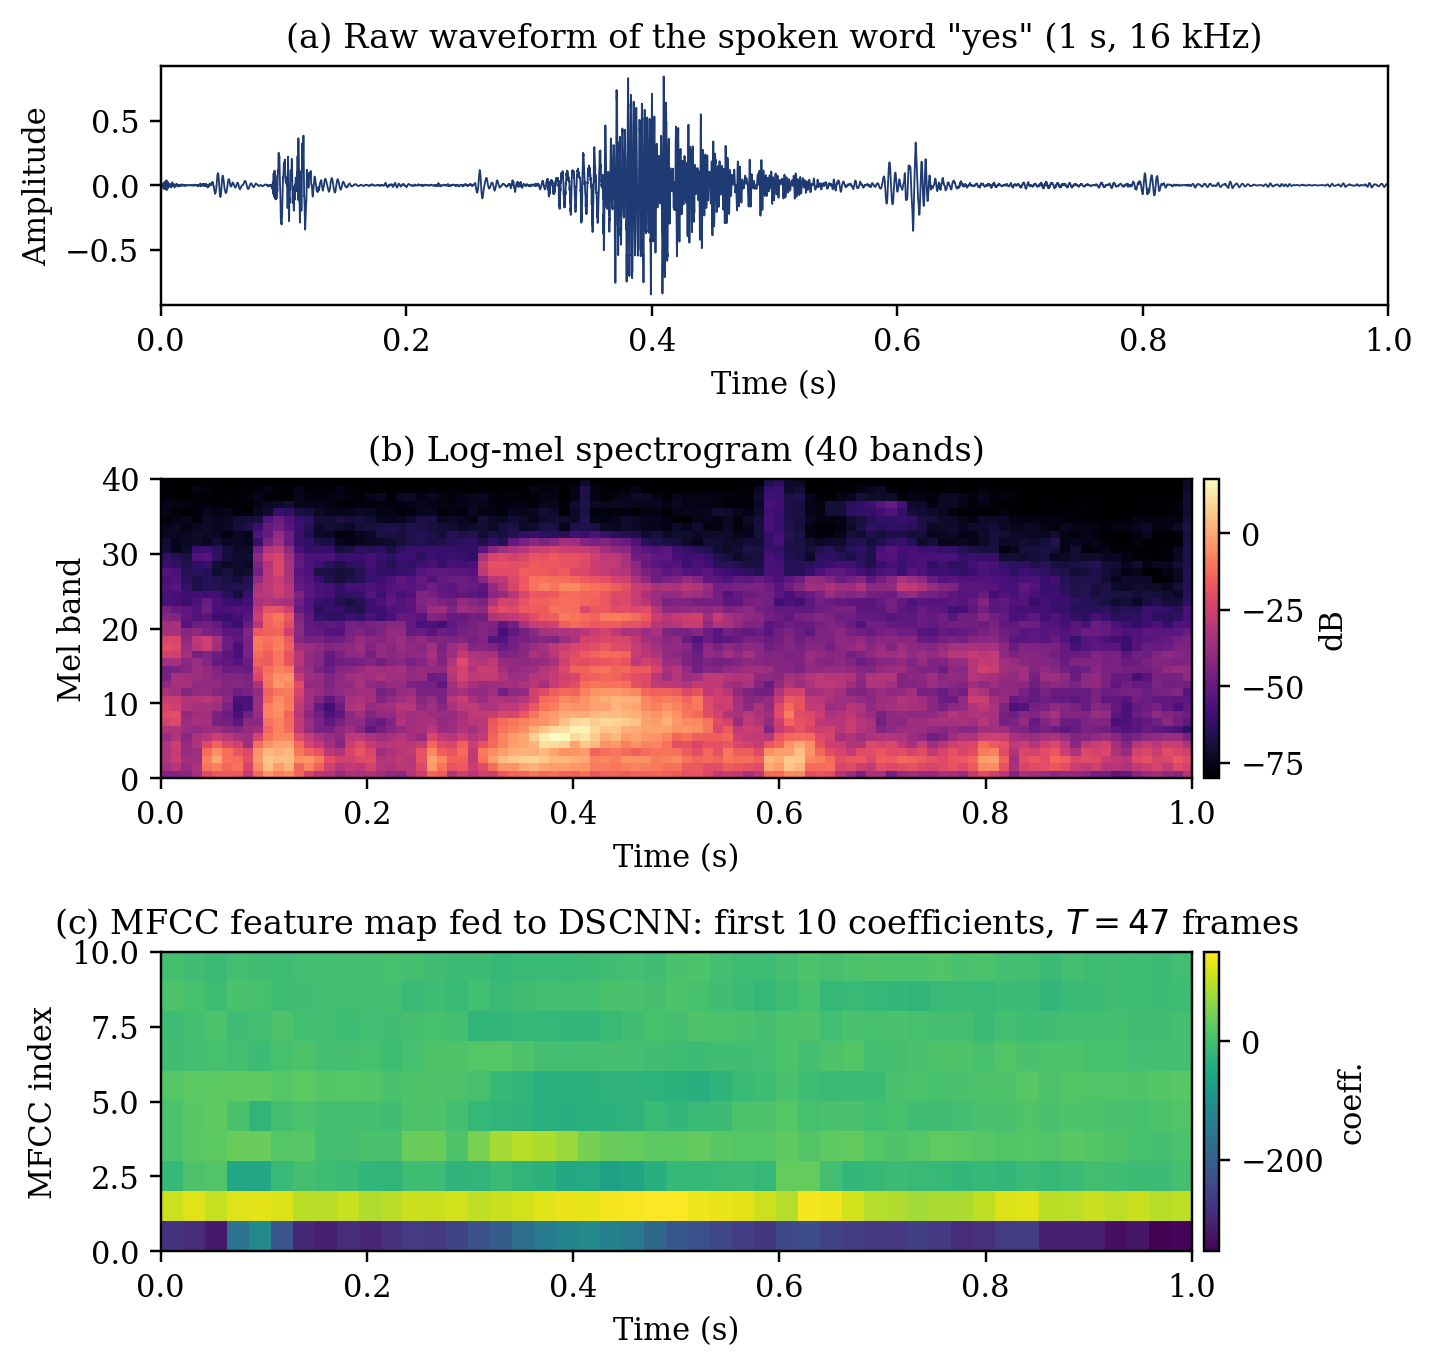
\includegraphics[width=0.92\linewidth]{fig_audio_features.png}
\caption{From sound to features, computed from a real Google Speech Commands
recording of the word ``yes''. (a) the 1\,s, 16\,kHz raw waveform; (b) the
40-band log-mel spectrogram; (c) the first 10 MFCC coefficients over $T{=}47$
frames --- the tensor actually fed to the DSCNN encoder.}
\label{fig:audiofeat}
\end{figure}

To build intuition for what the model sees, Figure~\ref{fig:dataexamples} shows
the log-mel spectrograms of six different command words. Each word has a
characteristic time--frequency signature --- the rising voiced segment of
``yes'', the plosive burst of ``stop'', the nasal onset of ``no'' --- and it is
this structure, not the raw waveform, that the encoder learns to compare.
Figure~\ref{fig:melfb} makes the mel front-end concrete: (a) the 40 overlapping
triangular filters, densely packed at low frequencies; and (b) the Hz-to-mel
warping of Equation~\eqref{eq:mel}.

\begin{figure}[t]
\centering
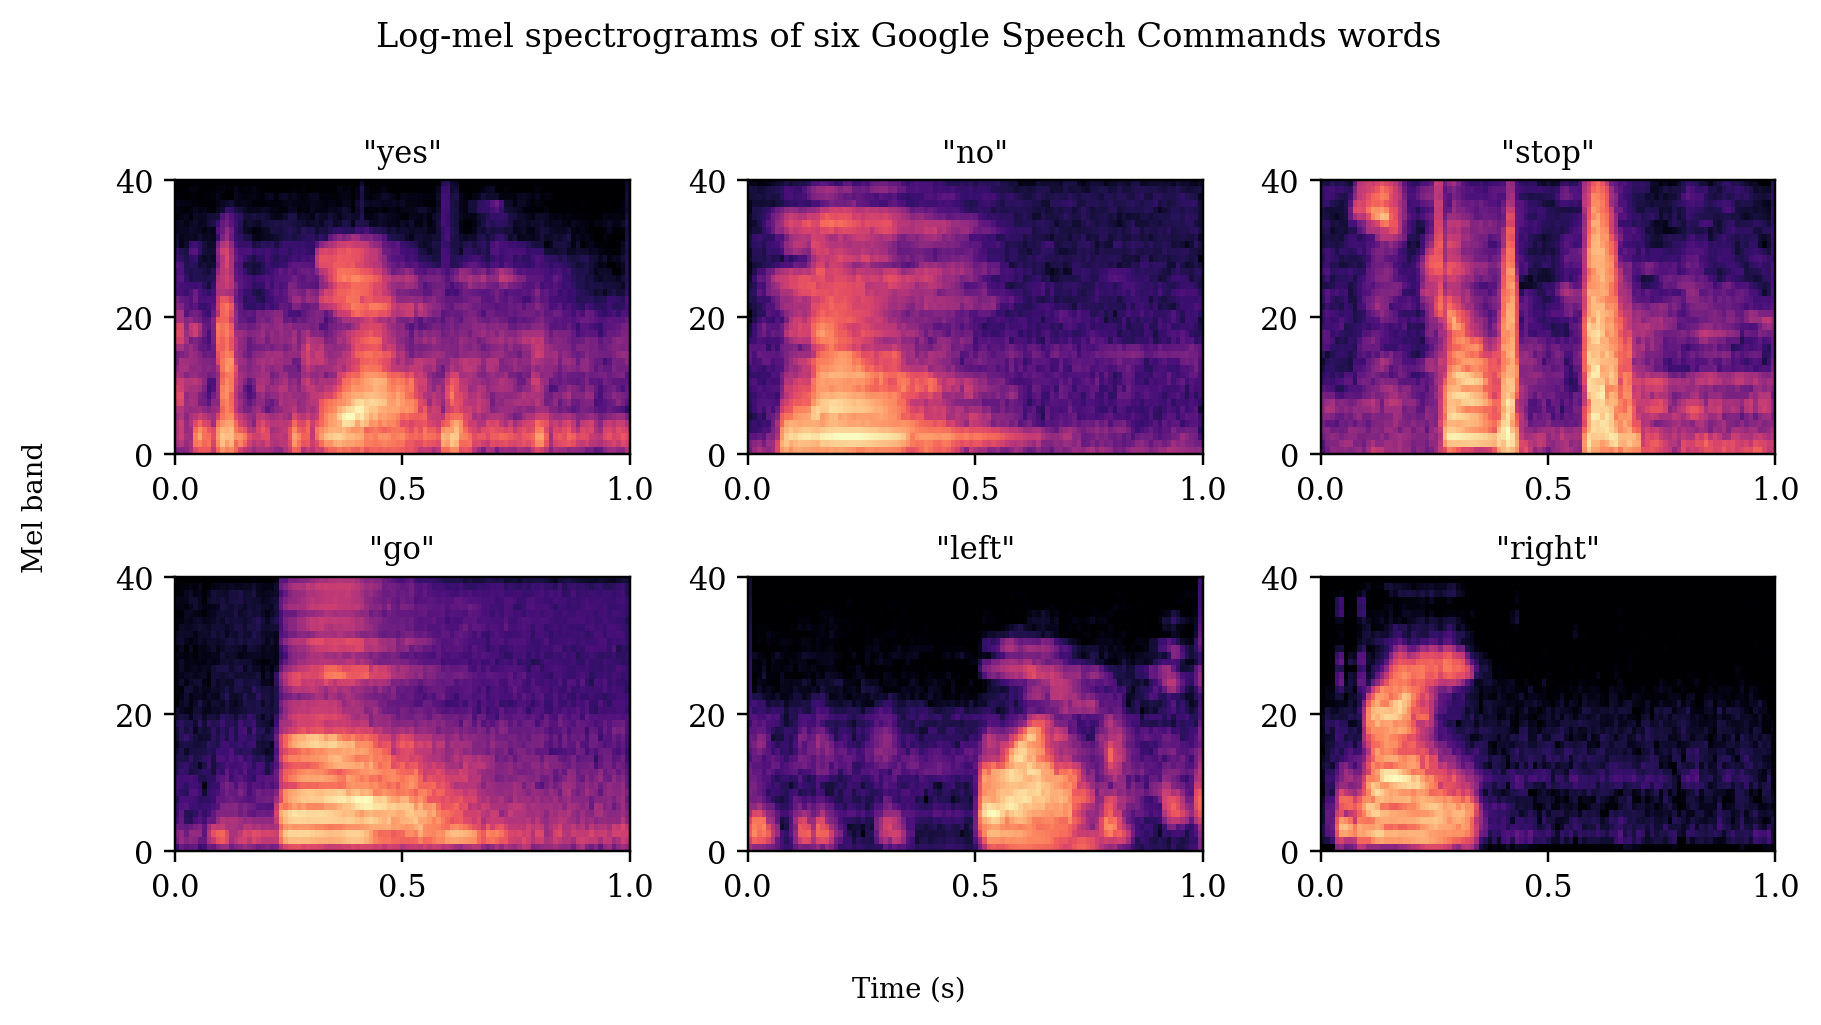
\includegraphics[width=0.95\linewidth]{fig_data_examples.png}
\caption{Log-mel spectrograms of six Google Speech Commands words (real data).
Different words occupy visibly different time--frequency patterns, which is what
makes metric learning in this space effective.}
\label{fig:dataexamples}
\end{figure}

\begin{figure}[t]
\centering
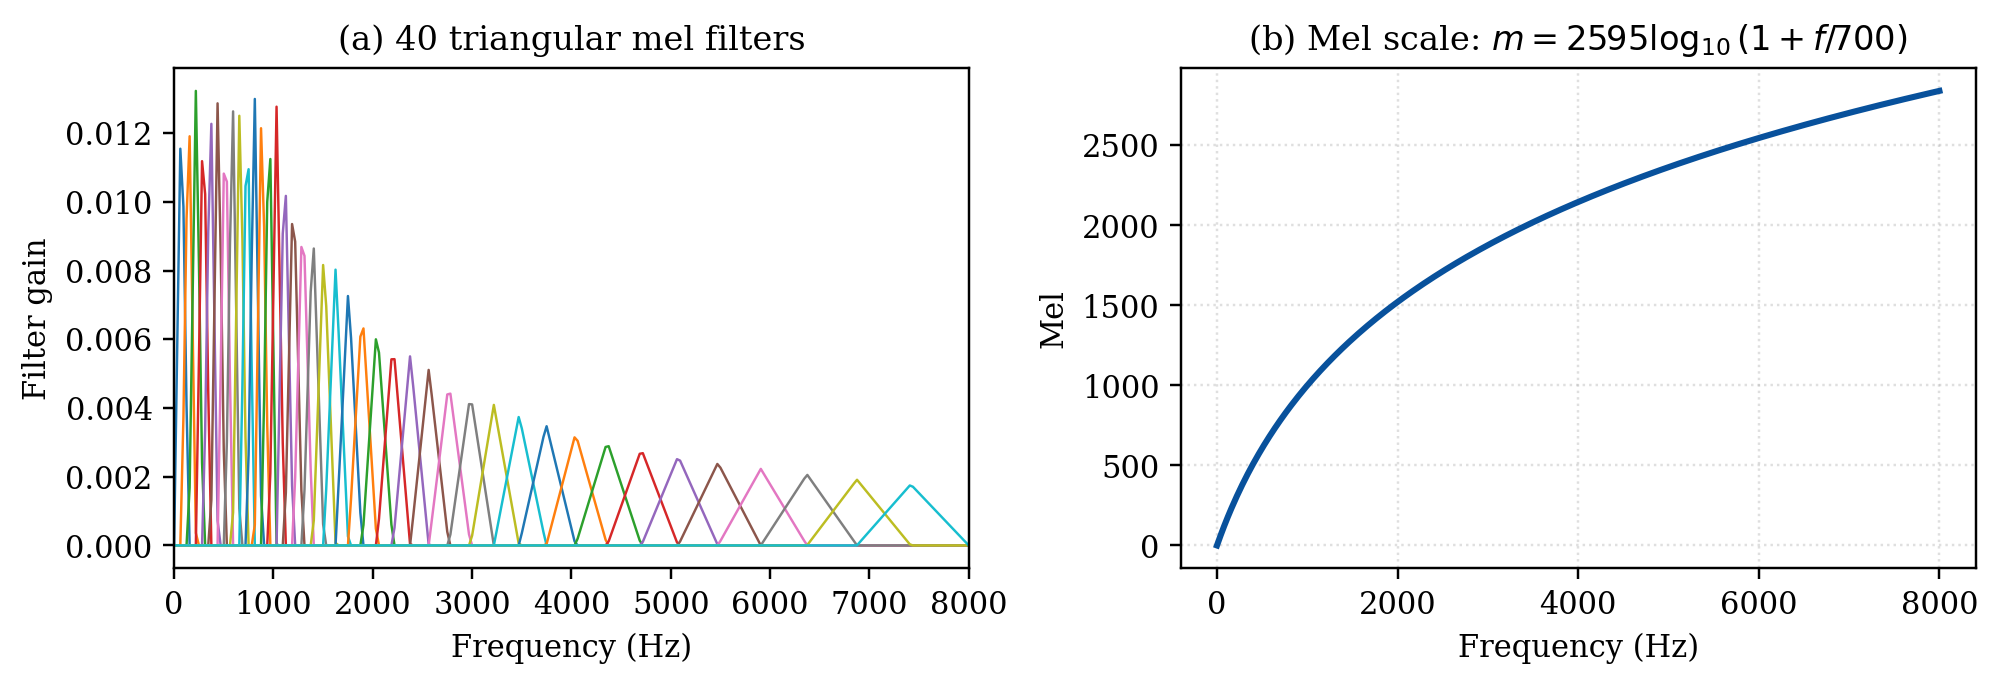
\includegraphics[width=0.95\linewidth]{fig_mel_filterbank.png}
\caption{The mel front-end. (a) the 40-channel triangular mel filterbank used in
this work; (b) the perceptual Hz$\to$mel warping curve.}
\label{fig:melfb}
\end{figure}

\subsection{Related work}\label{sec:related}

\paragraph{Small-footprint and open-set KWS.}
Small-footprint KWS was popularised by depthwise-separable convolutional networks
(DS-CNN)~\cite{zhang2017hello} and later refined by broadcasted-residual networks
(BC-ResNet)~\cite{kim2021bcresnet}, both trading accuracy against parameter count
for microcontroller deployment. These are \emph{closed-set} classifiers and
cannot, by design, abstain on unknown inputs. The open-set requirement ---
accepting known keywords while rejecting everything else --- is what separates a
laboratory accuracy number from a deployable wake-word engine.

\paragraph{Few-shot and metric learning.}
To support \emph{arbitrary} vocabularies we cast KWS as metric learning: the
network learns an embedding space in which utterances of the same word are close
and utterances of different words are far apart. Prototypical
networks~\cite{snell2017prototypical} represent each class by the mean of its few
support embeddings and classify queries by nearest prototype; triplet
embeddings~\cite{schroff2015facenet} optimise relative distances directly. The
Generalized End-to-End (GE2E) loss~\cite{wan2018ge2e}, originally proposed for
speaker verification, builds centroids inside each training batch exactly as
deployment builds prototypes, making it a natural fit for few-shot KWS.

\paragraph{Angular-margin classification, rejection, and self-supervision.}
ArcFace~\cite{deng2019arcface} and its sub-center variant
SCAF~\cite{deng2020subcenter} learn highly discriminative embeddings for face
recognition with thousands of identities by enforcing an angular margin. A
natural question --- which this thesis answers negatively at extreme scale --- is
whether the same machinery transfers to tens of thousands of word classes. For
the open-set decision itself, OpenMax~\cite{bendale2016openmax} fits Weibull
tails to per-class activations, and energy scores~\cite{liu2020energy} offer a
calibration-free alternative; we adapt both to operate on prototype distances and
compare them with a plain nearest-class-mean threshold. Finally, self-supervised
speech models such as Wav2Vec\,2.0~\cite{baevski2020wav2vec} provide powerful
representations; we use a frozen Wav2Vec\,2.0 only as a distillation
\emph{teacher}, keeping the deployed student tiny.

\subsection{Contributions}\label{sec:contrib}

\begin{itemize}[leftmargin=1.4em,itemsep=2pt]
\item A reproducible, dependency-light few-shot open-set KWS framework with two
compact encoders, three feature front-ends, four metric objectives, and four
open-set rejection heads, all sharing a common prototype interface.
\item A 16-configuration factorial screen on full-vocabulary MSWC that isolates
the contribution of each design axis with paired deltas; PCEN and GE2E emerge as
the two robust wins.
\item A scale analysis showing (a) accuracy saturation near $\sim$2\,M training
clips and (b) the failure mode of Sub-center ArcFace at $37$k classes, with a
gradient-magnitude explanation and a practical fix.
\item A knowledge-distillation study showing that a cosine objective against a
frozen Wav2Vec\,2.0 teacher matches GE2E accuracy with roughly half the training
data.
\item A complete cross-corpus evaluation under a strict 10-shot protocol (100
runs), plus a CPU streaming pipeline and an offline web demonstrator.
\end{itemize}

%==============================================================================
\section{Objectives}\label{sec:objectives}

\paragraph{Scientific objective.}
The objective of this internship is to design, implement, and rigorously evaluate
a \emph{retraining-free, open-set} keyword-spotting system that learns a single
transferable embedding and supports arbitrary user-defined vocabularies from a
few enrolment examples. The strategy is to (i) train one compact encoder on a
large word vocabulary with a deployment-matched metric objective, and (ii)
measure, through a controlled factorial study, which feature front-end, encoder
backbone, and metric-learning objective generalise best across corpora and how
they behave as the training vocabulary scales.

\paragraph{Concrete objectives.}
\begin{enumerate}[leftmargin=1.6em,itemsep=2pt]
\item Build a compact, dependency-light encoder that runs offline on modest
hardware ($\sim$0.1--0.4\,M parameters).
\item Identify, through a controlled factorial study, which front-end, backbone,
and objective generalise best across corpora.
\item Characterise how design choices behave as the training vocabulary scales
from tens to tens of thousands of words.
\item Deliver an honest open-set evaluation (DET/AUC/EER/ACC@FAR) under a strict,
reproducible protocol, plus a working streaming demonstrator.
\end{enumerate}

\paragraph{Desired outcomes.}
The system is expected to (i) recognise a user's own keyword set enrolled from
$\le 10$ examples per word without any retraining; (ii) reject out-of-vocabulary
speech and silence with a controllable false-accept rate; (iii) generalise across
recording conditions, demonstrated by training on one corpus (MSWC) and testing
on a different one (GSC); and (iv) remain small enough for offline, on-device use.

\paragraph{Research questions.}
The experiments are organised around four questions, which structure the results
in Section~\ref{sec:results}:
\begin{description}[leftmargin=1.8em,itemsep=2pt]
\item[\textbf{Q1 --- Which design axis matters?}] Train all
$2{\times}2{\times}4 = 16$ combinations of \{DSCNN-L, EdgeSpot-Full\} $\times$
\{MFCC, PCEN\} $\times$ \{Triplet, SCAF, GE2E, SCAF$+$GE2E\} and isolate each
axis with paired deltas.
\item[\textbf{Q2 --- How does performance scale?}] Fixing the best front-end and
loss, sweep the per-word cap $\{20,50,220,620\}$ and grow the vocabulary from 31
to $37{,}387$ words, watching for both saturation and failure.
\item[\textbf{Q3 --- Can distillation replace data?}] Compare GE2E against the
cosine-KD objective at matched data caps.
\item[\textbf{Q4 --- What is the best deployable system?}] Consolidate the
strongest configurations per data regime and identify the best overall and best
compact operating points.
\end{description}

%==============================================================================
\section{Materials and Methods}\label{sec:method}

At a high level (Figure~\ref{fig:pipeline}) the method has two phases that share a
single, frozen encoder. In the \emph{training phase} the encoder is optimised
once on MSWC with a metric objective. In the \emph{deployment phase} the user
enrols a few examples per keyword to form prototypes, and queries are recognised
by nearest-prototype distance with an explicit open-set threshold --- the encoder
is never retrained.

\begin{figure}[t]
\centering
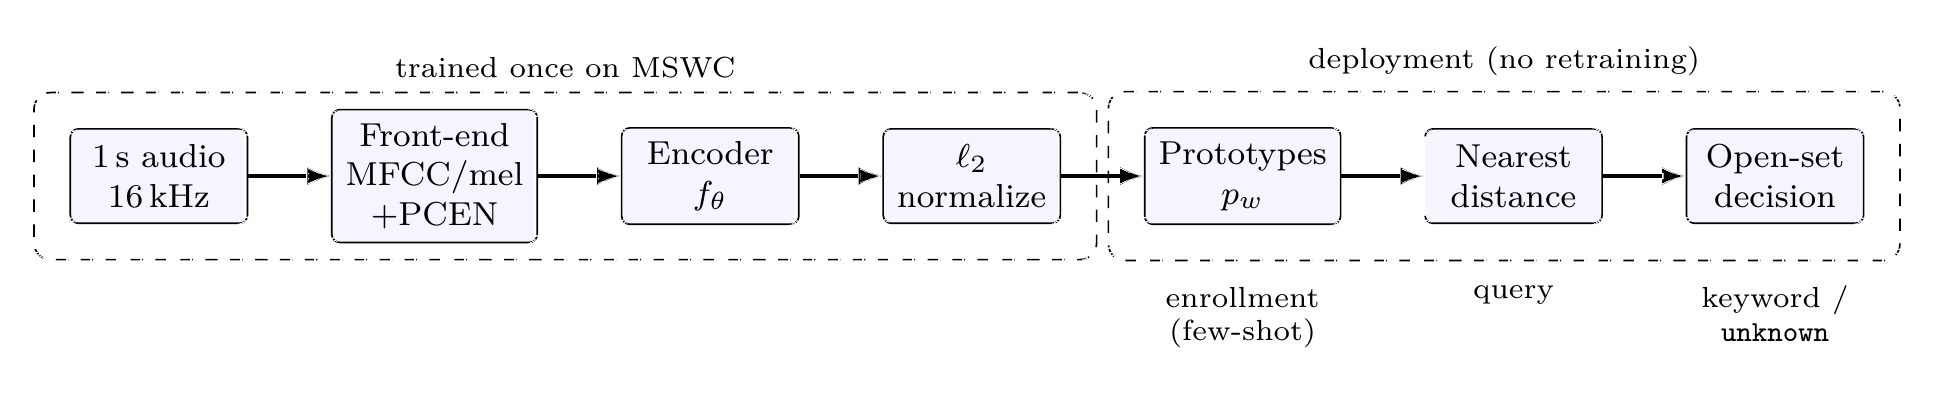
\includegraphics[width=0.98\linewidth]{fig_pipeline.png}
\caption{End-to-end few-shot open-set KWS pipeline. The encoder is trained once
on MSWC; at deployment, user keywords become prototypes and queries are
classified by nearest-prototype distance with an open-set threshold.}
\label{fig:pipeline}
\end{figure}

\subsection{Problem formulation}\label{sec:formulation}

Let $f_\theta:\mathbb{R}^{T\times F}\!\to\!\mathbb{R}^{d}$ be an encoder mapping a
one-second representation to a unit-norm embedding. The prototype of a keyword
$w$ is the mean of its $k$ support embeddings,
\begin{equation}
p_w \;=\; \frac{1}{k}\sum_{i=1}^{k} f_\theta\!\big(x^{(w)}_i\big).
\label{eq:proto}
\end{equation}
A query $x$ is assigned to the nearest prototype, with open-set score equal to the
negated minimum distance,
\begin{equation}
\hat w(x)=\arg\min_{w} d\!\big(f_\theta(x),p_w\big),\qquad
s(x)=-\!\min_{w} d\!\big(f_\theta(x),p_w\big),
\label{eq:score}
\end{equation}
and accepted as $\hat w(x)$ iff $s(x)\ge\tau$, otherwise labelled
\code{unknown}. Figure~\ref{fig:embedding} visualises the learned space:
running the best trained encoder on real GSC recordings and projecting embeddings
to two dimensions, each known command forms a tight, well-separated cluster
around its prototype (stars), while out-of-vocabulary words (grey crosses) fall
in the gaps --- exactly the geometry that makes nearest-prototype matching with
distance thresholding work for open-set rejection.

\begin{figure}[t]
\centering
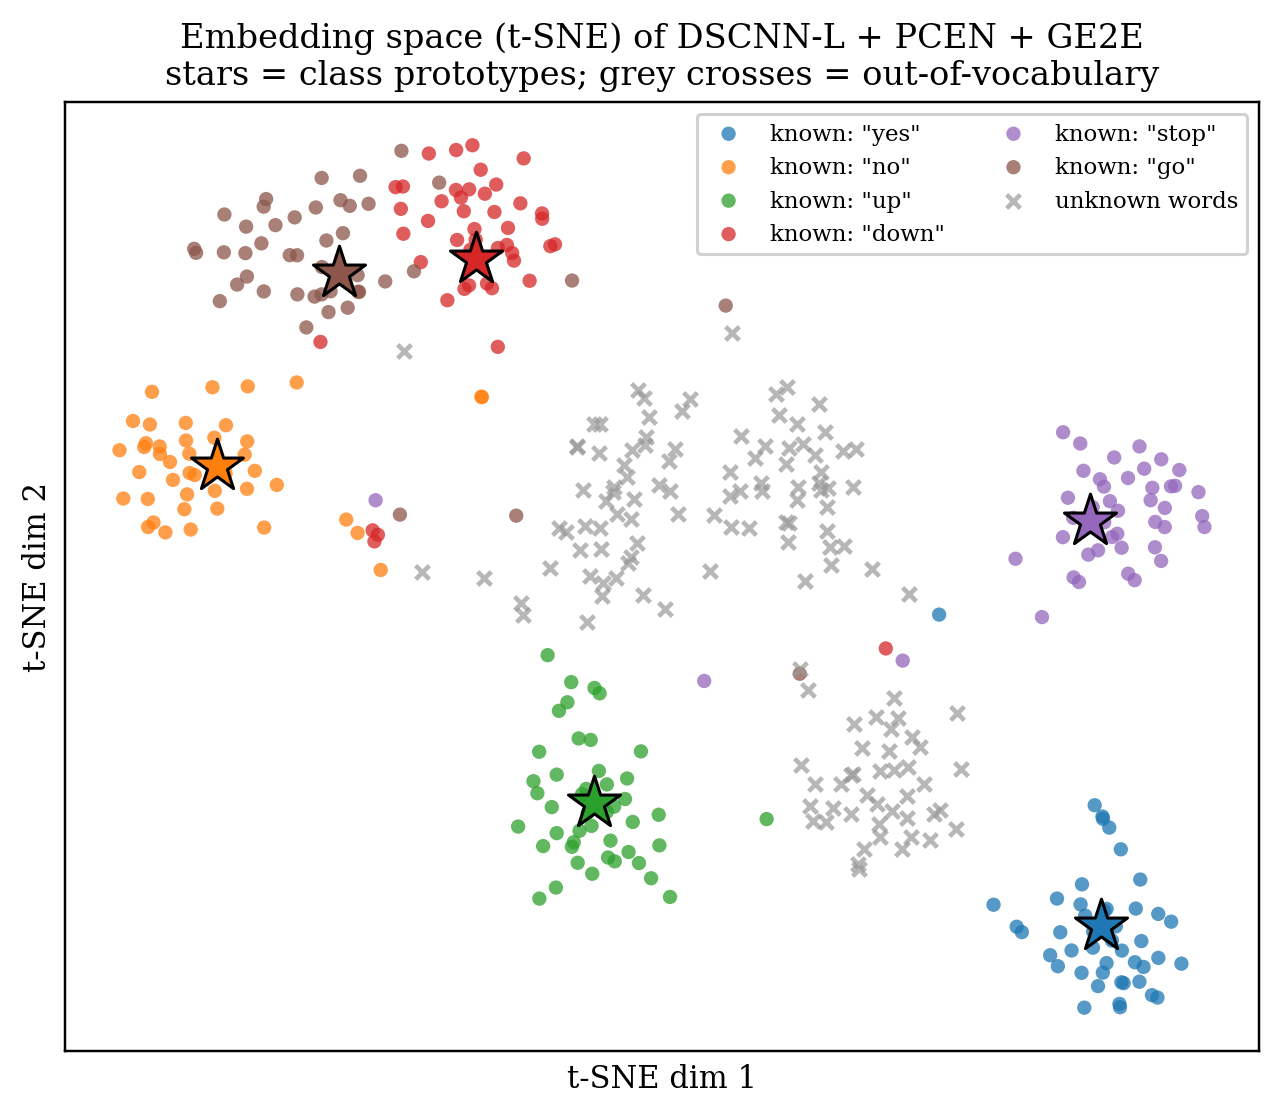
\includegraphics[width=0.86\linewidth]{fig_embedding_space.png}
\caption{t-SNE projection of embeddings from the trained DSCNN-L\,+\,PCEN\,+\,GE2E
model on real GSC audio. Coloured points are six known commands, stars are their
prototypes, grey crosses are out-of-vocabulary words.}
\label{fig:embedding}
\end{figure}

\subsection{Datasets and training protocol}\label{sec:data}

\textbf{Training corpus (MSWC English).} We train on the English subset of the
Multilingual Spoken Words Corpus~\cite{mazumder2021mswc}, which after filtering
for $\ge$ a minimum number of clips contains $37{,}387$ training words (and 763
validation words), drawn from a metadata pool of $\sim$38,150 words and
$\sim$6.6\,M clips. To study scale we form caps of $\{20, 50, 220, 620\}$ clips
per word --- roughly $\{0.53, 0.94, 2.05, 2.99\}$\,M training clips --- and two
reduced regimes: a Top-500 legacy split (450 train / 50 val words) and an
MLCommons micro-set (31 keywords) used only for pipeline validation and
architecture screening. The three vocabulary regimes span more than three orders
of magnitude (Figure~\ref{fig:vocabscale}); this range is what makes the scale
effects in Section~\ref{sec:results} observable.

\begin{figure}[t]
\centering
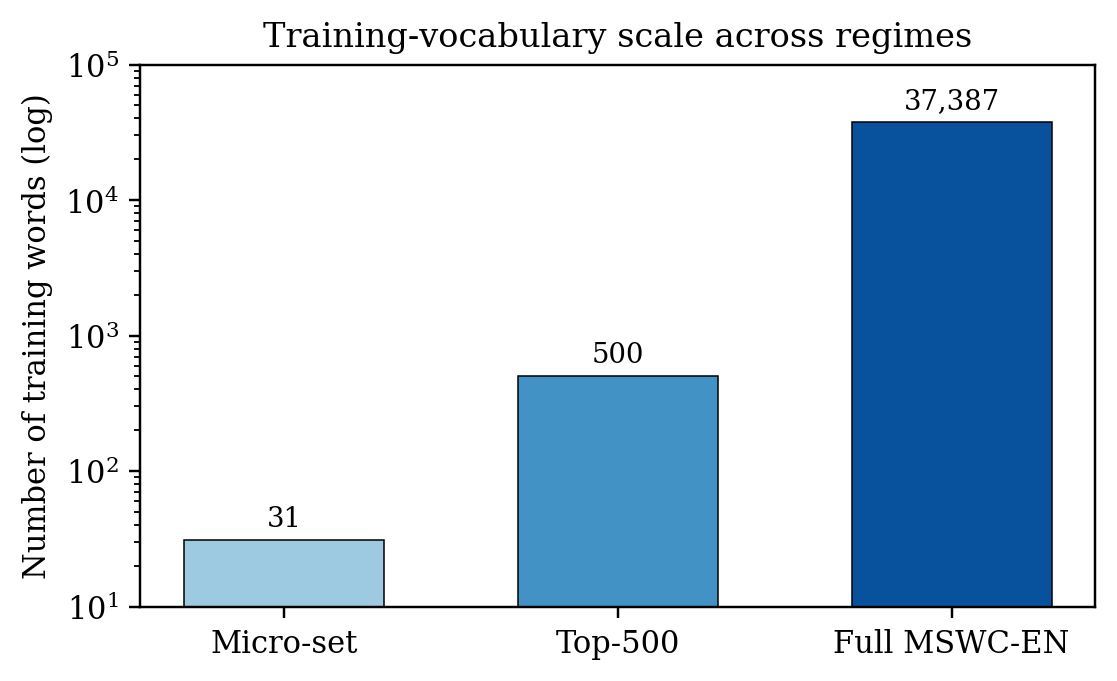
\includegraphics[width=0.72\linewidth]{fig_vocab_scale.png}
\caption{Training-vocabulary size for the three regimes (log scale). The
micro-set is used only for screening; full MSWC English is the headline regime.}
\label{fig:vocabscale}
\end{figure}

\textbf{Episodic sampling and augmentation.} Episodes draw 30 classes $\times$ 20
utterances (only classes with $\ge 20$ clips are eligible). Online augmentation
mixes DEMAND background noise (probability 0.5, SNR sampled in $[0, 10]$\,dB) and
applies SpecAugment (one frequency mask of width 6, one time mask of width 8);
gain perturbation ($\pm6$\,dB) and time-shift ($\le 100$\,ms) are applied with
probability 0.5. Figure~\ref{fig:augment} illustrates these augmentations on a
real recording.

\begin{figure}[t]
\centering
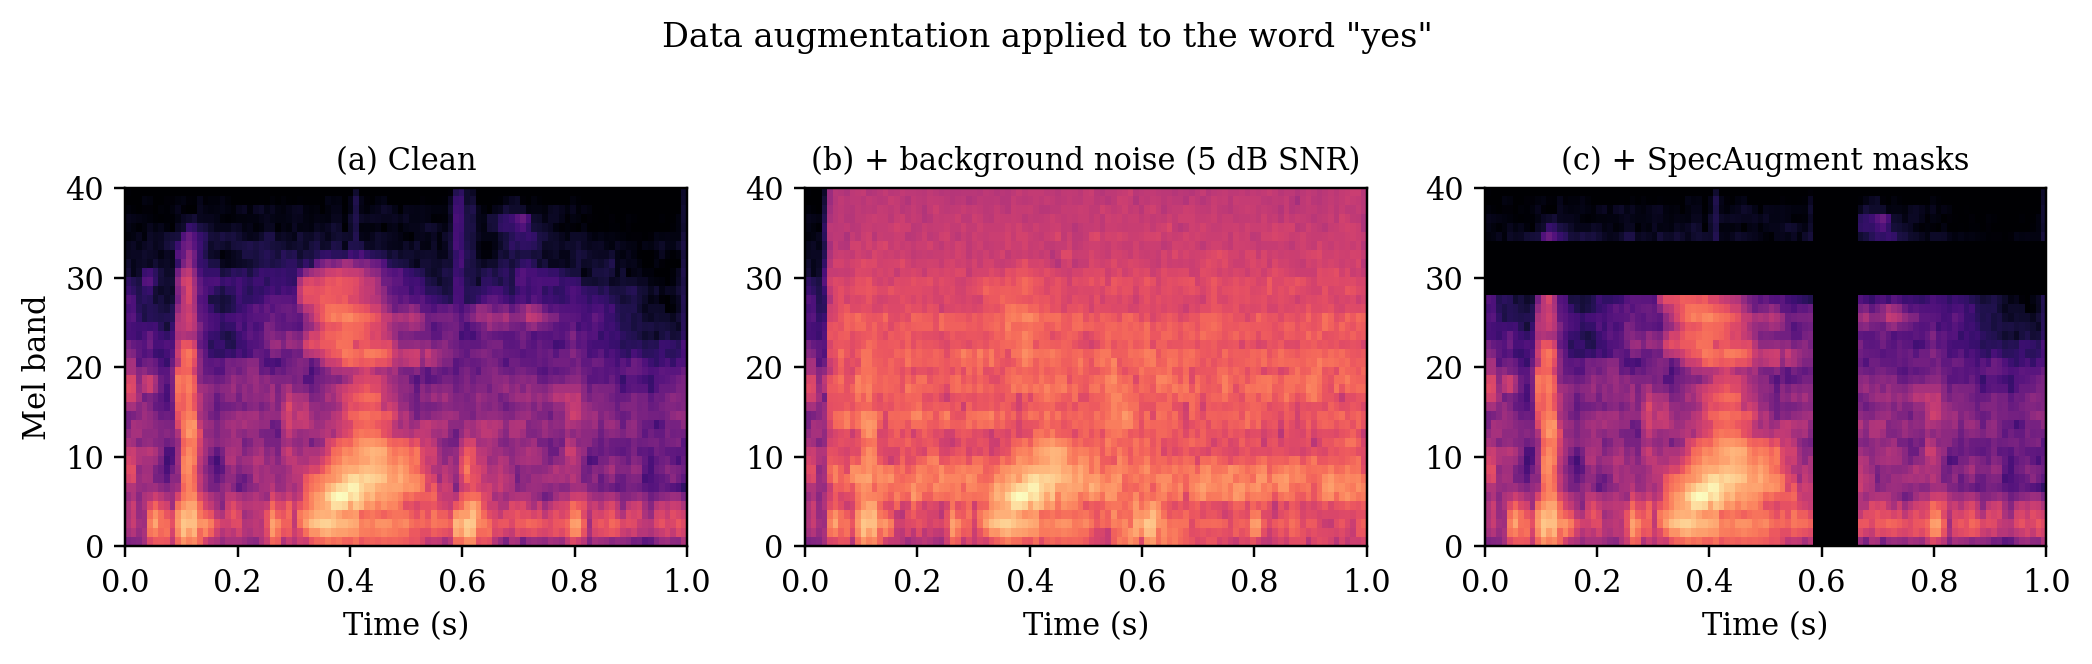
\includegraphics[width=0.98\linewidth]{fig_augmentation.png}
\caption{Training-time augmentation on the word ``yes'' (real data): (a) clean
log-mel; (b) $+$ real background noise at 5\,dB SNR; (c) $+$ SpecAugment frequency
and time masks.}
\label{fig:augment}
\end{figure}

\textbf{Evaluation corpus (GSC v2).} We evaluate cross-corpus on Google Speech
Commands v2~\cite{warden2018speech}. Enrolment (support) samples are drawn from
the official \code{validation\_list.txt}; query samples from
\code{testing\_list.txt} (``test'') or the remaining files (``dev''), preventing
leakage. A synthetic \code{\_silence\_} class is generated from random one-second
crops of \code{\_background\_noise\_}, with disjoint crops for support and query.

\textbf{Open-set protocol.} The headline protocol partitions GSC's 35 words into
11 positive classes --- the ten command words \{yes, no, up, down, left, right,
on, off, stop, go\} plus \code{\_silence\_} --- and 25 negative (unknown) spoken
words. Each run enrols $k{=}10$ shots per positive word, computes prototypes, and
scores up to 50 query samples per word (a fixed-seed subsample). We report the
mean$\pm$std over 100 randomised runs; randomness comes from enrolment-shot
selection. ``test100'' denotes 100 runs on the test split, ``dev30'' denotes 30
runs on the dev split.

\subsection{Feature front-ends}\label{sec:frontends}

All audio is mono, 16\,kHz, and trimmed/zero-padded to exactly one second
($16{,}000$ samples). We support two spectral parameterisations
(Table~\ref{tab:features}).

\begin{table}[t]
\centering
\caption{Feature front-end configurations.}
\label{tab:features}
\begin{tabular}{lcc}
\toprule
 & \textbf{MFCC} & \textbf{Log-mel} \\
\midrule
Sample rate     & \multicolumn{2}{c}{16\,kHz, mono, 1\,s} \\
FFT size        & 1024  & 512  \\
Window / hop    & 40/20\,ms & 25/10\,ms \\
\code{center}   & \code{False} & \code{True} \\
Mel bands       & 40 & 40 \\
Output coeffs.  & 10 (first DCT) & 40 (mel) \\
Tensor shape    & $(1,47,10)$ & $(1,40,101)$ \\
Trainable PCEN  & optional & optional \\
\bottomrule
\end{tabular}
\end{table}

\textbf{MFCC (DSCNN front-end).} We compute 40 Mel-frequency cepstral
coefficients with a 1024-point FFT, 640-sample (40\,ms) Hann window, 320-sample
(20\,ms) hop, and \code{center=False}; the Mel filterbank uses Slaney scale and
Slaney area normalisation, and the log is taken as $10\log_{10}(\cdot)$ followed
by an orthonormal DCT-II. We retain only the first 10 coefficients and transpose
to a tensor of shape $(1,47,10)$, where $T = 47 =
\lfloor(16000-1024)/320\rfloor + 1$.

\textbf{Log-mel (EdgeSpot front-end).} We use 40 Mel bands with a 512-point FFT,
400-sample (25\,ms) window, 160-sample (10\,ms) hop, and \code{center=True},
producing $(1,40,101)$. The log compression is delegated to the PCEN layer.

\textbf{Trainable PCEN.} Per-channel energy
normalisation~\cite{wang2017trainable} applies a causal first-order IIR smoother
$M_t = (1-s)M_{t-1} + sE_t$ followed by adaptive gain and dynamic-range
compression,
\begin{equation}
\text{PCEN}(E_t)=\Big(\frac{E_t}{(\epsilon+M_t)^{\alpha}}+\delta\Big)^{r}-\delta^{r},
\label{eq:pcen}
\end{equation}
with learnable $\alpha,\delta,r,s$ (initialised to $0.96, 2.0, 0.5, 0.04$;
$\epsilon{=}10^{-6}$). PCEN replaces the static log and adapts to channel
statistics during training.

\subsection{Encoders}\label{sec:encoders}

\textbf{DSCNN-L.} A depthwise-separable CNN: an initial
$\text{Conv}(1{\to}276, 10{\times}4, \text{stride } 2{\times}1)$ with
TensorFlow-style asymmetric ``same'' padding, followed by five depthwise
separable blocks (276 channels, $3{\times}3$ kernels; the first strides
$2{\times}2$). All but the last block use BatchNorm$+$ReLU; the last uses an
affine-free LayerNorm. A global average pool yields the embedding directly, so
the embedding dimension equals the channel width, $d = 276$ (no final linear
projection). DSCNN-L has $\approx 0.413$\,M parameters
(Figure~\ref{fig:dscnn}).

\textbf{EdgeSpot-Full ($\tau{=}4$).} A width-scaled edge encoder on the
$(1,40,101)$ mel/PCEN input. A $5{\times}5$ stride-$(2,1)$ stem feeds four stages
of fused-temporal and broadcasted-residual ``lite'' blocks with increasing
temporal dilation $(1,2,4,8)$; a depthwise frequency-collapse block averages over
frequency to a $(C,T)$ sequence; a depthwise positional convolution and a
single-head temporal self-attention block ($d{=}64$) model long-range temporal
structure; a depthwise temporal head and global pooling produce a 64-dimensional
embedding. EdgeSpot-Full $\tau{=}4$ has $\approx 0.131$\,M parameters,
$\sim$3.2$\times$ smaller than DSCNN-L (Figure~\ref{fig:edgespot}).

\begin{table}[t]
\centering
\caption{Encoder comparison. $\ell_2$-normalisation is applied outside the
encoder so all losses and the deployment classifier operate on the hypersphere.}
\label{tab:encoders}
\begin{tabular}{lccc}
\toprule
\textbf{Encoder} & \textbf{Front-end} & \textbf{$d$} & \textbf{Params} \\
\midrule
DSCNN-L              & MFCC / mel($+$PCEN) & 276 & 0.413\,M \\
EdgeSpot-Full $\tau{=}4$ & mel($+$PCEN)    & 64  & 0.131\,M \\
EdgeSpot-Lite       & mel($+$PCEN)        & 64  & $<0.131$\,M \\
BC-ResNet-FS $\tau{=}4$  & mel($+$PCEN)    & 64  & $\sim$0.1\,M \\
\bottomrule
\end{tabular}
\end{table}

\begin{figure}[t]
\centering
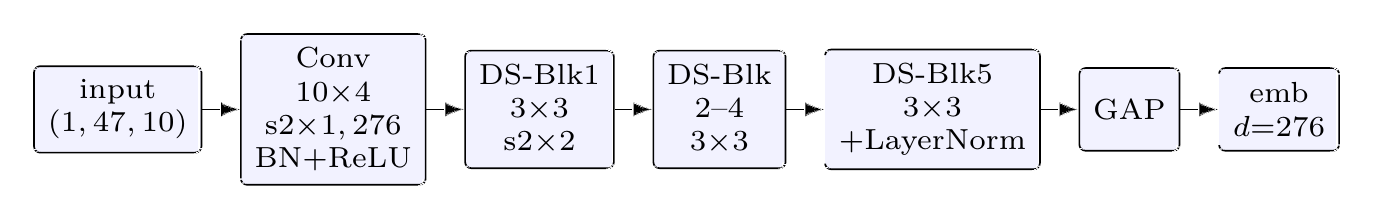
\includegraphics[width=0.95\linewidth]{fig_dscnn_arch.png}
\caption{DSCNN-L encoder: depthwise-separable CNN, $\approx$0.41\,M parameters.
The embedding equals the final channel width (276); no linear projection.}
\label{fig:dscnn}
\end{figure}

\begin{figure}[t]
\centering
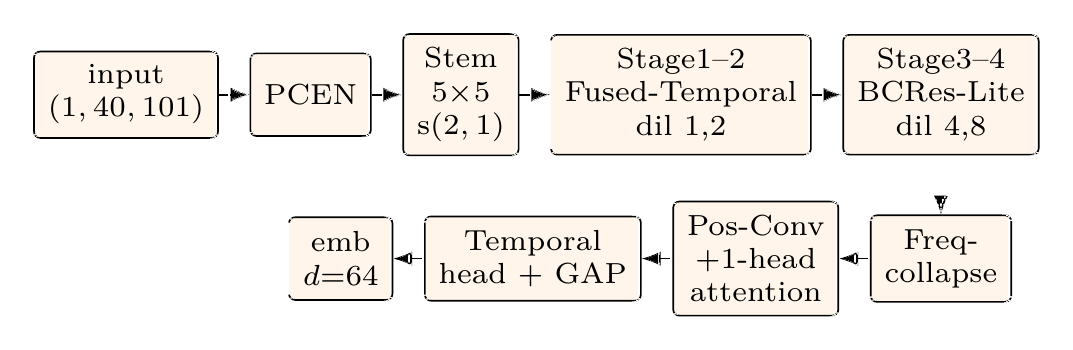
\includegraphics[width=0.85\linewidth]{fig_edgespot_arch.png}
\caption{EdgeSpot-Full ($\tau{=}4$) encoder: mel/PCEN front-end, fused-temporal
and broadcasted-residual blocks with growing dilation, frequency collapse, and a
single-head temporal self-attention stage, $\approx$0.13\,M parameters.}
\label{fig:edgespot}
\end{figure}

\subsection{Metric-learning objectives}\label{sec:losses}

All objectives are trained episodically: each episode samples 30 classes with 20
utterances each (600 embeddings/episode).

\textbf{Triplet.} Semi-hard triplet loss~\cite{schroff2015facenet} with Euclidean
distance, $\mathcal{L}=\frac{1}{N}\sum\max(0, d(a,p)-d(a,n)+m)$, with
hardest-positive and FaceNet semi-hard negative mining.

\textbf{Sub-center ArcFace (SCAF).} An angular-margin softmax with $K{=}3$
sub-centers per class. With normalised weights, the per-class logit is the max
cosine over its sub-centers, $\cos\theta_c = \max_{j\le K} w_{c,j}^{\top} z$; the
additive margin $m{=}0.5$ is applied to the target class and logits are scaled by
$s{=}30$ before cross-entropy.

\textbf{GE2E (centroid).} Generalised end-to-end loss~\cite{wan2018ge2e} that
mirrors deployment: within an episode each class is split into support/query; the
centroid is the $\ell_2$-normalised support mean and queries are classified by
scaled cosine similarity to all centroids, optimised by cross-entropy. GE2E
directly optimises the enrol-then-match objective of
Equations~\eqref{eq:proto}--\eqref{eq:score}.

\textbf{Cosine knowledge distillation (KD).} We distil from a frozen
Wav2Vec\,2.0-base teacher~\cite{baevski2020wav2vec} (hidden layer 16, mean-pooled,
projected to $d{=}64$). The distillation loss is a pure embedding-cosine term,
\begin{equation}
\mathcal{L}_{\text{KD}} = 1 - \frac{1}{N}\sum_i
\cos\!\big(f_\theta(x_i),\, g_{\text{teacher}}(x_i)\big),
\label{eq:kd}
\end{equation}
with no temperature/soft-label term. Teacher embeddings are precomputed offline
and looked up by file path during training.

\textbf{Hybrid combinations.} We form weighted sums (e.g.\ \code{scaf\_ge2e},
\code{kd\_ge2e}). A crucial implementation detail (and a key empirical finding,
Section~\ref{sec:results}) is the SCAF weight: under KD it is set to
$5\times10^{-5}$ while GE2E/KD weights are 1.0, preventing the high-magnitude
angular-margin classification loss from dominating the centroid/cosine terms.

\textbf{Optimisation.} Unless noted, training uses Adam (learning rate
$10^{-3}$, weight decay $10^{-4}$), gradient clipping at $5.0$, a
cosine-annealing-with-warm-restarts schedule ($T_0{=}10$, $T_{\text{mult}}{=}2$,
$\eta_{\min}{=}10^{-5}$), and a fixed seed (42) with cuDNN determinism.

\subsection{Open-set rejection heads}\label{sec:openset}

All heads share the prototype interface and differ only in the rejection score;
the predicted keyword is always the argmin-distance class
(Equation~\eqref{eq:score}). (i) \textbf{Nearest-class-mean (NCM, ``Direct
$\ell_2$'')} --- our default --- rejects when the minimum prototype distance
exceeds a threshold. (ii) \textbf{OpenMax}~\cite{bendale2016openmax} fits a
Weibull tail to support-to-prototype distances and uses $1-\mathrm{CDF}$ as the
membership score. (iii) \textbf{Energy}~\cite{liu2020energy} treats $-d_i$ as
logits and uses the free energy $E(x)=T\log\sum_i\exp(-d_i/T)$ as the acceptance
score. (iv) \textbf{Calibrated} thresholds ($\mu+2\sigma$ of support distances)
drive per-word confusion analysis.

\subsection{Evaluation methodology}\label{sec:eval}

We treat the open-set problem as binary keyword-vs-non-keyword detection
augmented by a multiclass identity track, and build all metrics on the ROC.
\begin{itemize}[leftmargin=1.3em,itemsep=1pt]
\item \textbf{AUC:} area under the ROC of the open-set scores; threshold-free.
\item \textbf{EER:} equal-error rate, the operating point minimising
$|\text{FAR}-\text{FRR}|$, reported as $(\text{FAR}+\text{FRR})/2$.
\item \textbf{FRR@FAR:} false-reject rate at the largest threshold whose
false-accept rate does not exceed the target (1\% or 5\%).
\item \textbf{Open-set ACC@FAR:} the headline accuracy. A known query is correct
iff it is accepted ($s\ge\tau_{\text{FAR}}$) and the argmin label is correct; an
unknown query is correct iff it is rejected. Reported at FAR\,$\in\{1\%, 5\%\}$.
\item \textbf{Keyword ACC:} closed-set nearest-prototype accuracy over known
queries only (ignores rejection).
\item \textbf{F1:} binary keyword-vs-unknown F1 at the EER threshold.
\end{itemize}

\textbf{Interpretation caveat.} AUC and EER are threshold-free, whereas ACC@FAR
and FRR@FAR use a threshold derived from the evaluation ROC (an oracle operating
point), not transferred from a held-out calibration split. We therefore treat
ACC@FAR as a comparison metric across systems under matched conditions, and
report AUC/EER/F1 jointly so that degenerate operating points are visible: a
system that rejects nearly everything scores high open-set ACC against many
negatives while missing all positives, and such cases are exposed by
$\text{FRR}\to100\%$ and $\text{F1}\to0$.

\subsection{Deployment: streaming and demonstrator}\label{sec:deploy}

Beyond the core encoder, the system includes a CPU streaming pipeline and an
offline web demonstrator. Streaming performs sliding-window detection (1\,s
window) gated by Silero Voice Activity Detection (VAD): only windows that VAD
marks as speech are embedded and matched, reducing computation and false
activations on silence. A backend-agnostic decision \emph{state machine}
(Appendix~A) stabilises raw candidates into clean events using majority-vote
smoothing over a short window, a top-2 margin check, and a cooldown to suppress
duplicate firings. The streaming server decouples audio ingestion from inference
(a non-blocking receiver feeds a single-inference-at-a-time consumer on a fixed
cadence), which bounds end-to-end detection latency under load without changing
the detection arithmetic. Optional modules --- a spectral-gating denoiser and an
ECAPA-TDNN speaker-verification gate --- follow the same fail-open, runtime-toggle
pattern.

\TODOfig{A screenshot of the offline web demonstrator (model switcher plus
long-audio timing view), exported from the local demo at $1280\times720$ and
saved as \code{assets/demo\_ui.png}.}

%==============================================================================
\section{Results and Discussion}\label{sec:results}

All numbers are mean$\pm$std over the 10-shot open-set protocol (100 runs on GSC
test, denoted test100). Higher is better for ACC/AUC/F1/Keyword-ACC; lower is
better for EER/FRR.

\subsection{Training dynamics}\label{sec:res-train}

Figure~\ref{fig:traincurves} shows the real training trajectory of the Microset
anchor model (EdgeSpot-Full + SCAF+GE2E), read directly from saved TensorBoard
logs. The loss decreases smoothly from $\sim$15.5 to $\sim$1.3, the validation
AUC rises to and stabilises near $98\%$, and the GSC-dev open-set accuracy
plateaus around $85\%$ --- a healthy, non-overfitting trajectory. The contrasting
\emph{collapse} behaviour at full $37$k-class vocabulary is discussed in
Section~\ref{sec:res-q2}.

\begin{figure}[t]
\centering
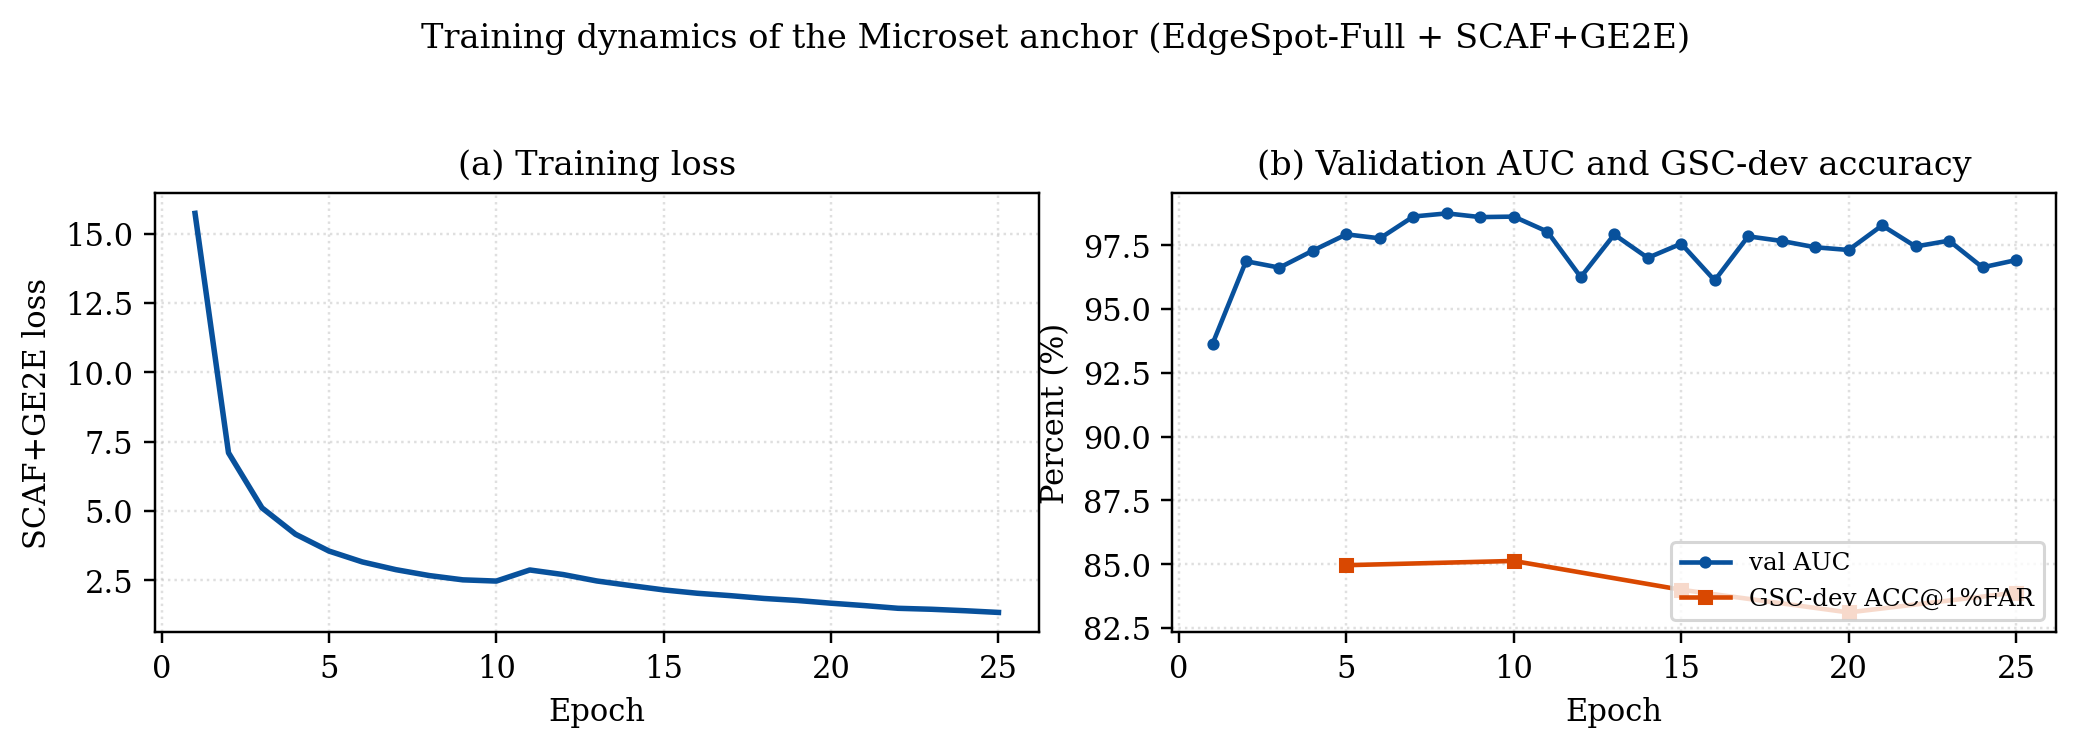
\includegraphics[width=0.98\linewidth]{fig_training_curves.png}
\caption{Real training dynamics of the Microset anchor (EdgeSpot-Full +
SCAF+GE2E), from local TensorBoard logs: (a) training loss; (b) validation AUC
and GSC-dev ACC@1\%FAR over epochs.}
\label{fig:traincurves}
\end{figure}

\subsection{Q1: Which design axis matters}\label{sec:res-q1}

Table~\ref{tab:matrix} reports the full 16-configuration screen on full-vocabulary
MSWC (cap-620), and Figure~\ref{fig:ranked} ranks the configurations visually. Two
findings are immediate: PCEN-based pipelines occupy the top of the ranking, and
the centroid GE2E loss is the best objective for every backbone. The
classification objective SCAF (and the SCAF$+$GE2E hybrid at full weight)
collapses at this scale --- analysed in Section~\ref{sec:res-q2}.

\begin{table}[t]
\centering
\caption{Full 16-configuration screen on full-vocabulary MSWC (cap-620), GSC
test100 @ 1\% FAR. ``coll.'' marks degenerate collapse (AUC$=$50, F1$=$0,
FRR$=$100\%). Best in bold.}
\label{tab:matrix}
\small
\setlength{\tabcolsep}{5pt}
\begin{tabular}{lll r r r r}
\toprule
\textbf{Enc.} & \textbf{Feat.} & \textbf{Loss} &
ACC$_{1\%}$ & AUC & EER & F1\\
\midrule
DSCNN & MFCC & Triplet     & 71.52 & 75.55 & 31.41 & 57.17 \\
DSCNN & MFCC & SCAF        & 70.08 & 55.04 & 46.41 & 41.38 \\
DSCNN & MFCC & GE2E        & 77.08 & 86.46 & 21.95 & 68.50 \\
DSCNN & MFCC & SCAF+GE2E   & 69.04 & 47.78 & 52.15 & 35.93 \\
DSCNN & PCEN & Triplet     & 79.98 & 90.65 & 17.57 & 74.14 \\
DSCNN & PCEN & SCAF        & 69.44 & 50.00 & 50.00 & coll. \\
\rowcolor{blue!7}
DSCNN & PCEN & GE2E        & \textbf{82.34} & \textbf{92.42} & \textbf{14.89} & \textbf{77.75} \\
DSCNN & PCEN & SCAF+GE2E   & 69.44 & 50.00 & 50.00 & coll. \\
Edge  & MFCC & Triplet     & 69.63 & 52.84 & 48.05 & 39.79 \\
Edge  & MFCC & SCAF        & 69.44 & 50.00 & 50.00 & coll. \\
Edge  & MFCC & GE2E        & 70.76 & 65.30 & 39.05 & 48.82 \\
Edge  & MFCC & SCAF+GE2E   & 69.67 & 50.88 & 50.39 & 37.57 \\
Edge  & PCEN & Triplet     & 79.58 & 89.85 & 18.22 & 73.29 \\
Edge  & PCEN & SCAF        & 69.44 & 50.00 & 50.00 & coll. \\
\rowcolor{blue!7}
Edge  & PCEN & GE2E        & \textbf{79.98} & 87.23 & 20.23 & 70.68 \\
Edge  & PCEN & SCAF+GE2E   & 69.44 & 50.00 & 50.00 & coll. \\
\bottomrule
\end{tabular}
\end{table}

\begin{figure}[t]
\centering
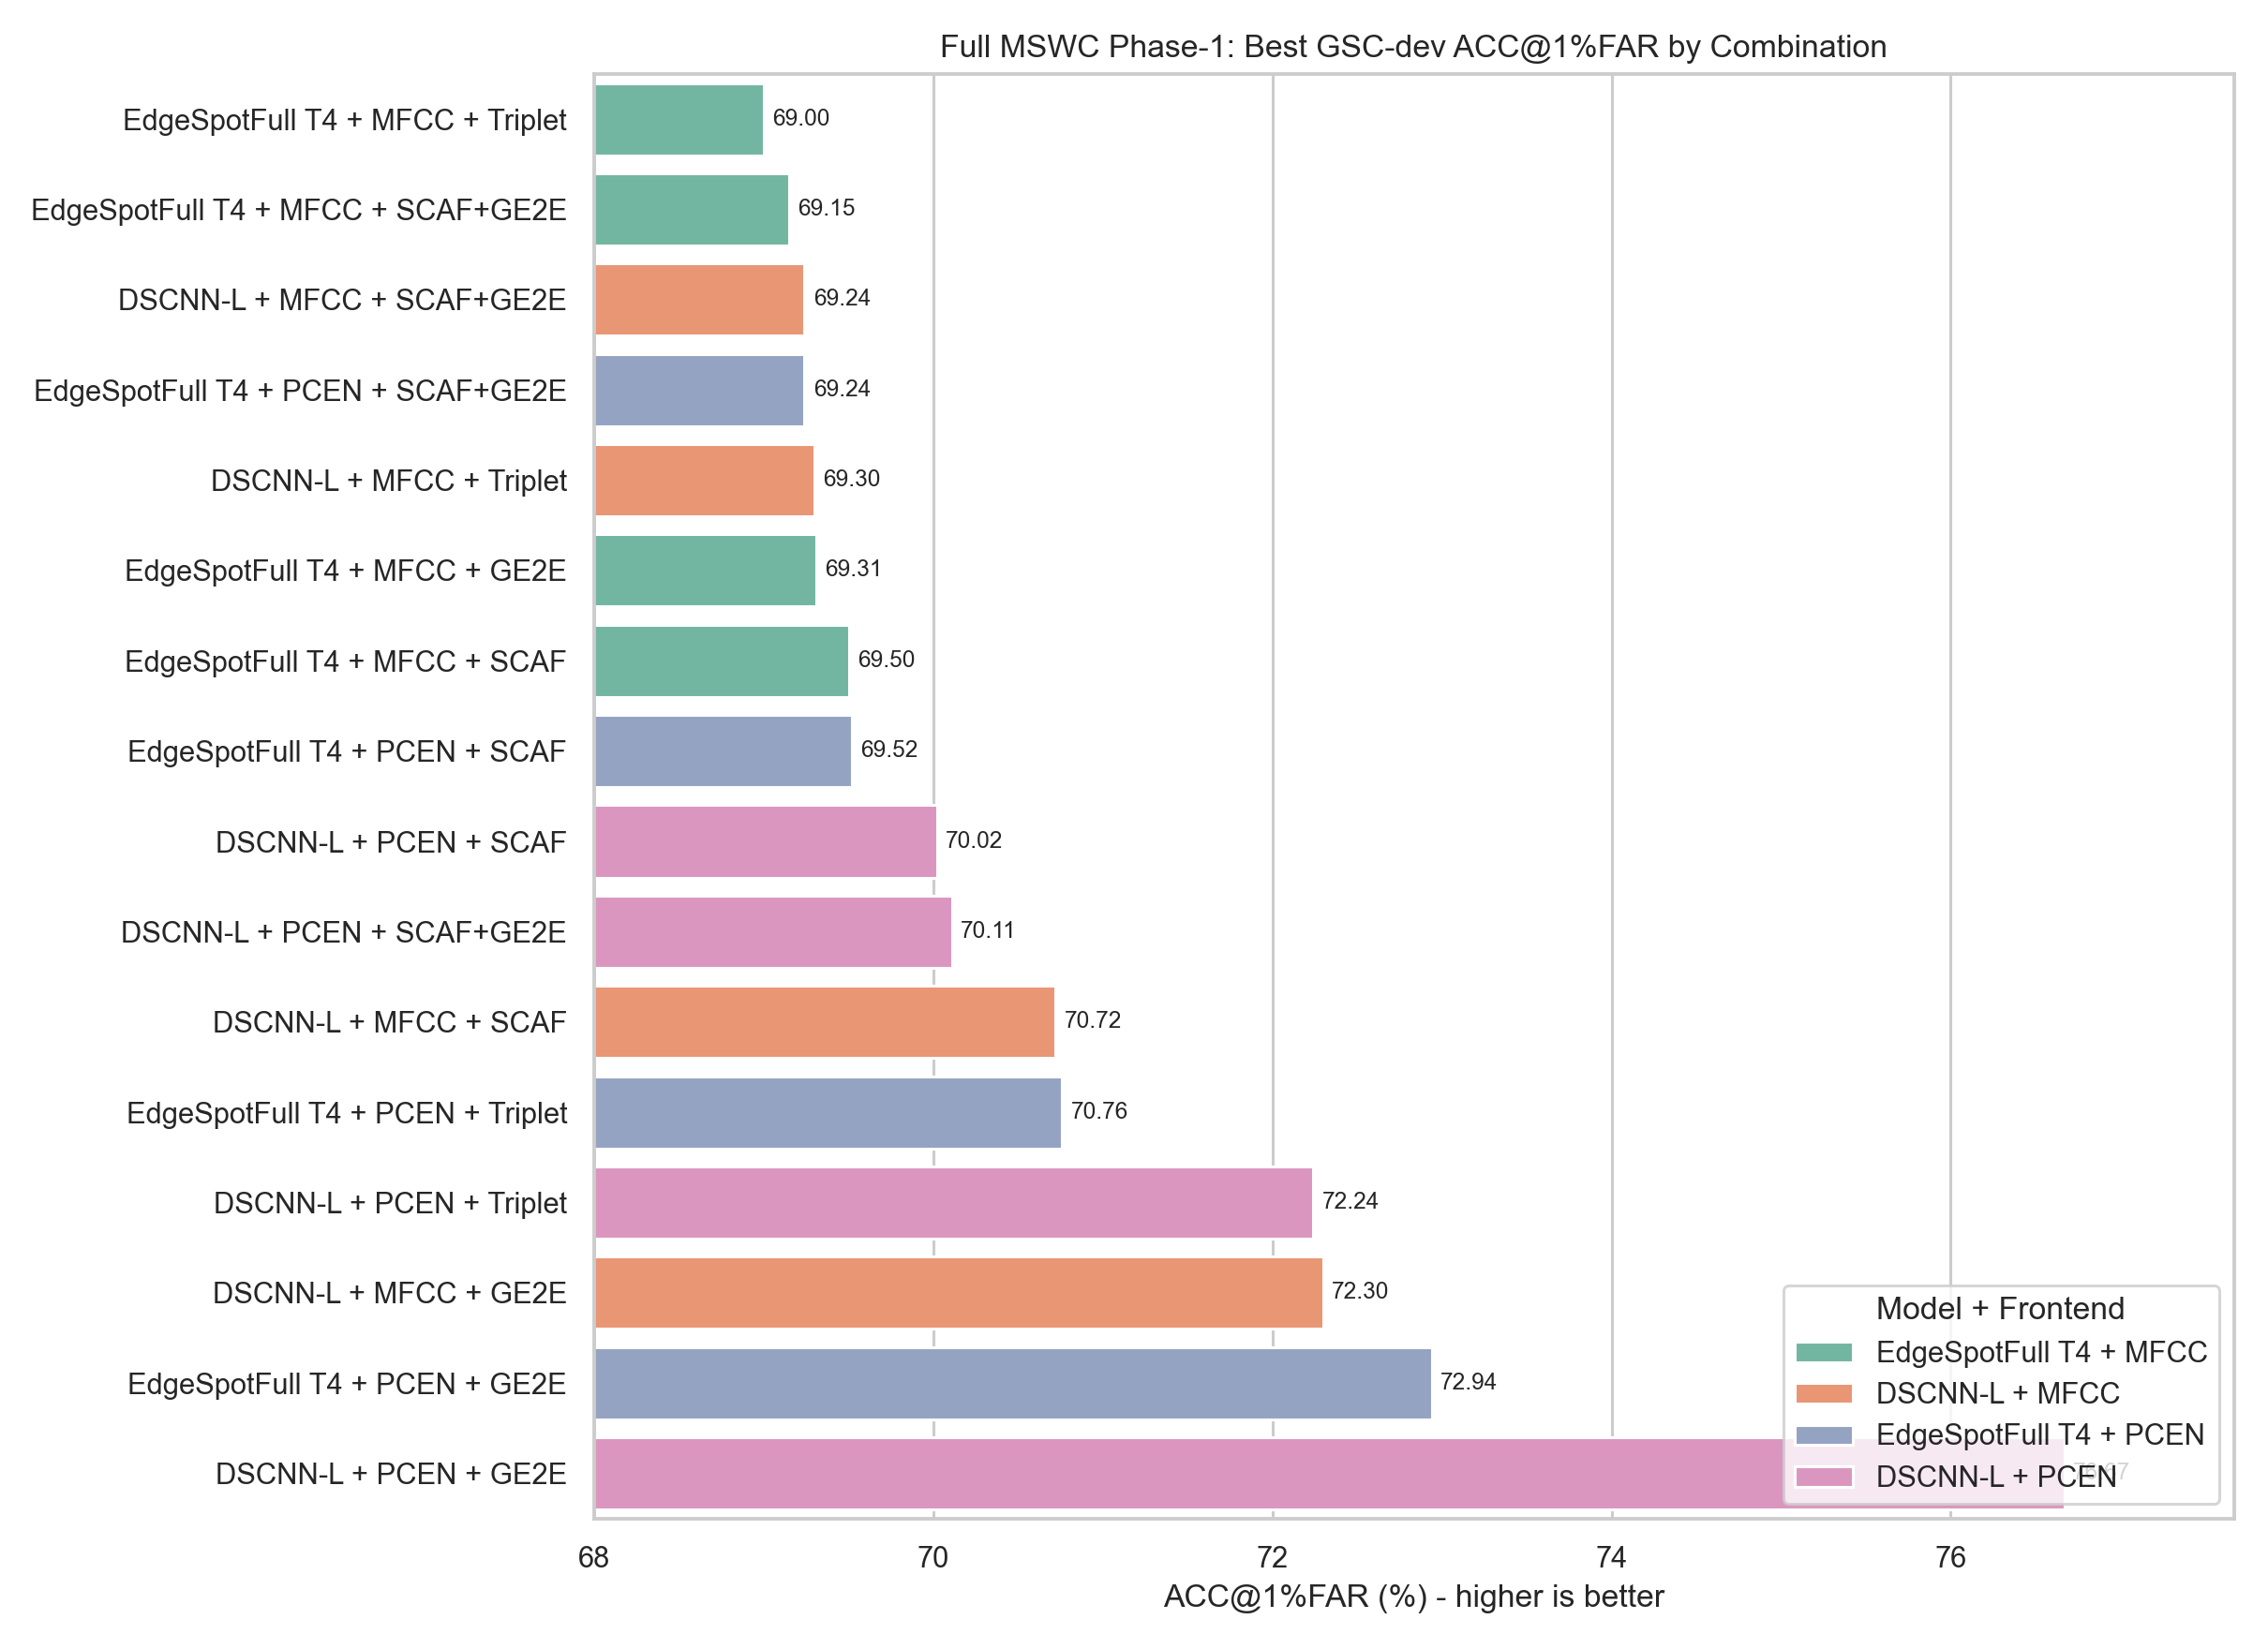
\includegraphics[width=0.96\linewidth]{res_ranked_bar.png}
\caption{Configurations ranked by GSC ACC@1\%FAR (phase-1 screen on full MSWC).
PCEN$+$GE2E pipelines lead; colour encodes backbone$\times$front-end.}
\label{fig:ranked}
\end{figure}

\paragraph{Paired effect deltas.}
Isolating each axis (Table~\ref{tab:deltas}, Figure~\ref{fig:deltas}) shows two
robust wins. PCEN improves every backbone --- most dramatically the edge encoder
($+9.22$ ACC, $+21.86$ F1) --- and GE2E consistently beats triplet. The front-end
therefore carries proportionally more of the representational burden when the
backbone is small.

\begin{table}[t]
\centering
\caption{Paired effect deltas (percentage points), full-vocabulary MSWC, GSC
test100 @ 1\% FAR. Positive favours the first option.}
\label{tab:deltas}
\small
\begin{tabular}{l r r r}
\toprule
\textbf{Contrast (others fixed)} & $\Delta$ACC$_{1\%}$ & $\Delta$AUC & $\Delta$F1\\
\midrule
PCEN $-$ MFCC \;(DSCNN, GE2E)    & +5.26 & +5.96  & +9.25 \\
PCEN $-$ MFCC \;(Edge, GE2E)     & +9.22 & +21.93 & +21.86 \\
GE2E $-$ Triplet \;(DSCNN, PCEN) & +2.36 & +1.77  & +3.61 \\
DSCNN $-$ Edge \;(PCEN, GE2E)    & +2.36 & +5.19  & +7.07 \\
\bottomrule
\end{tabular}
\end{table}

\begin{figure}[t]
\centering
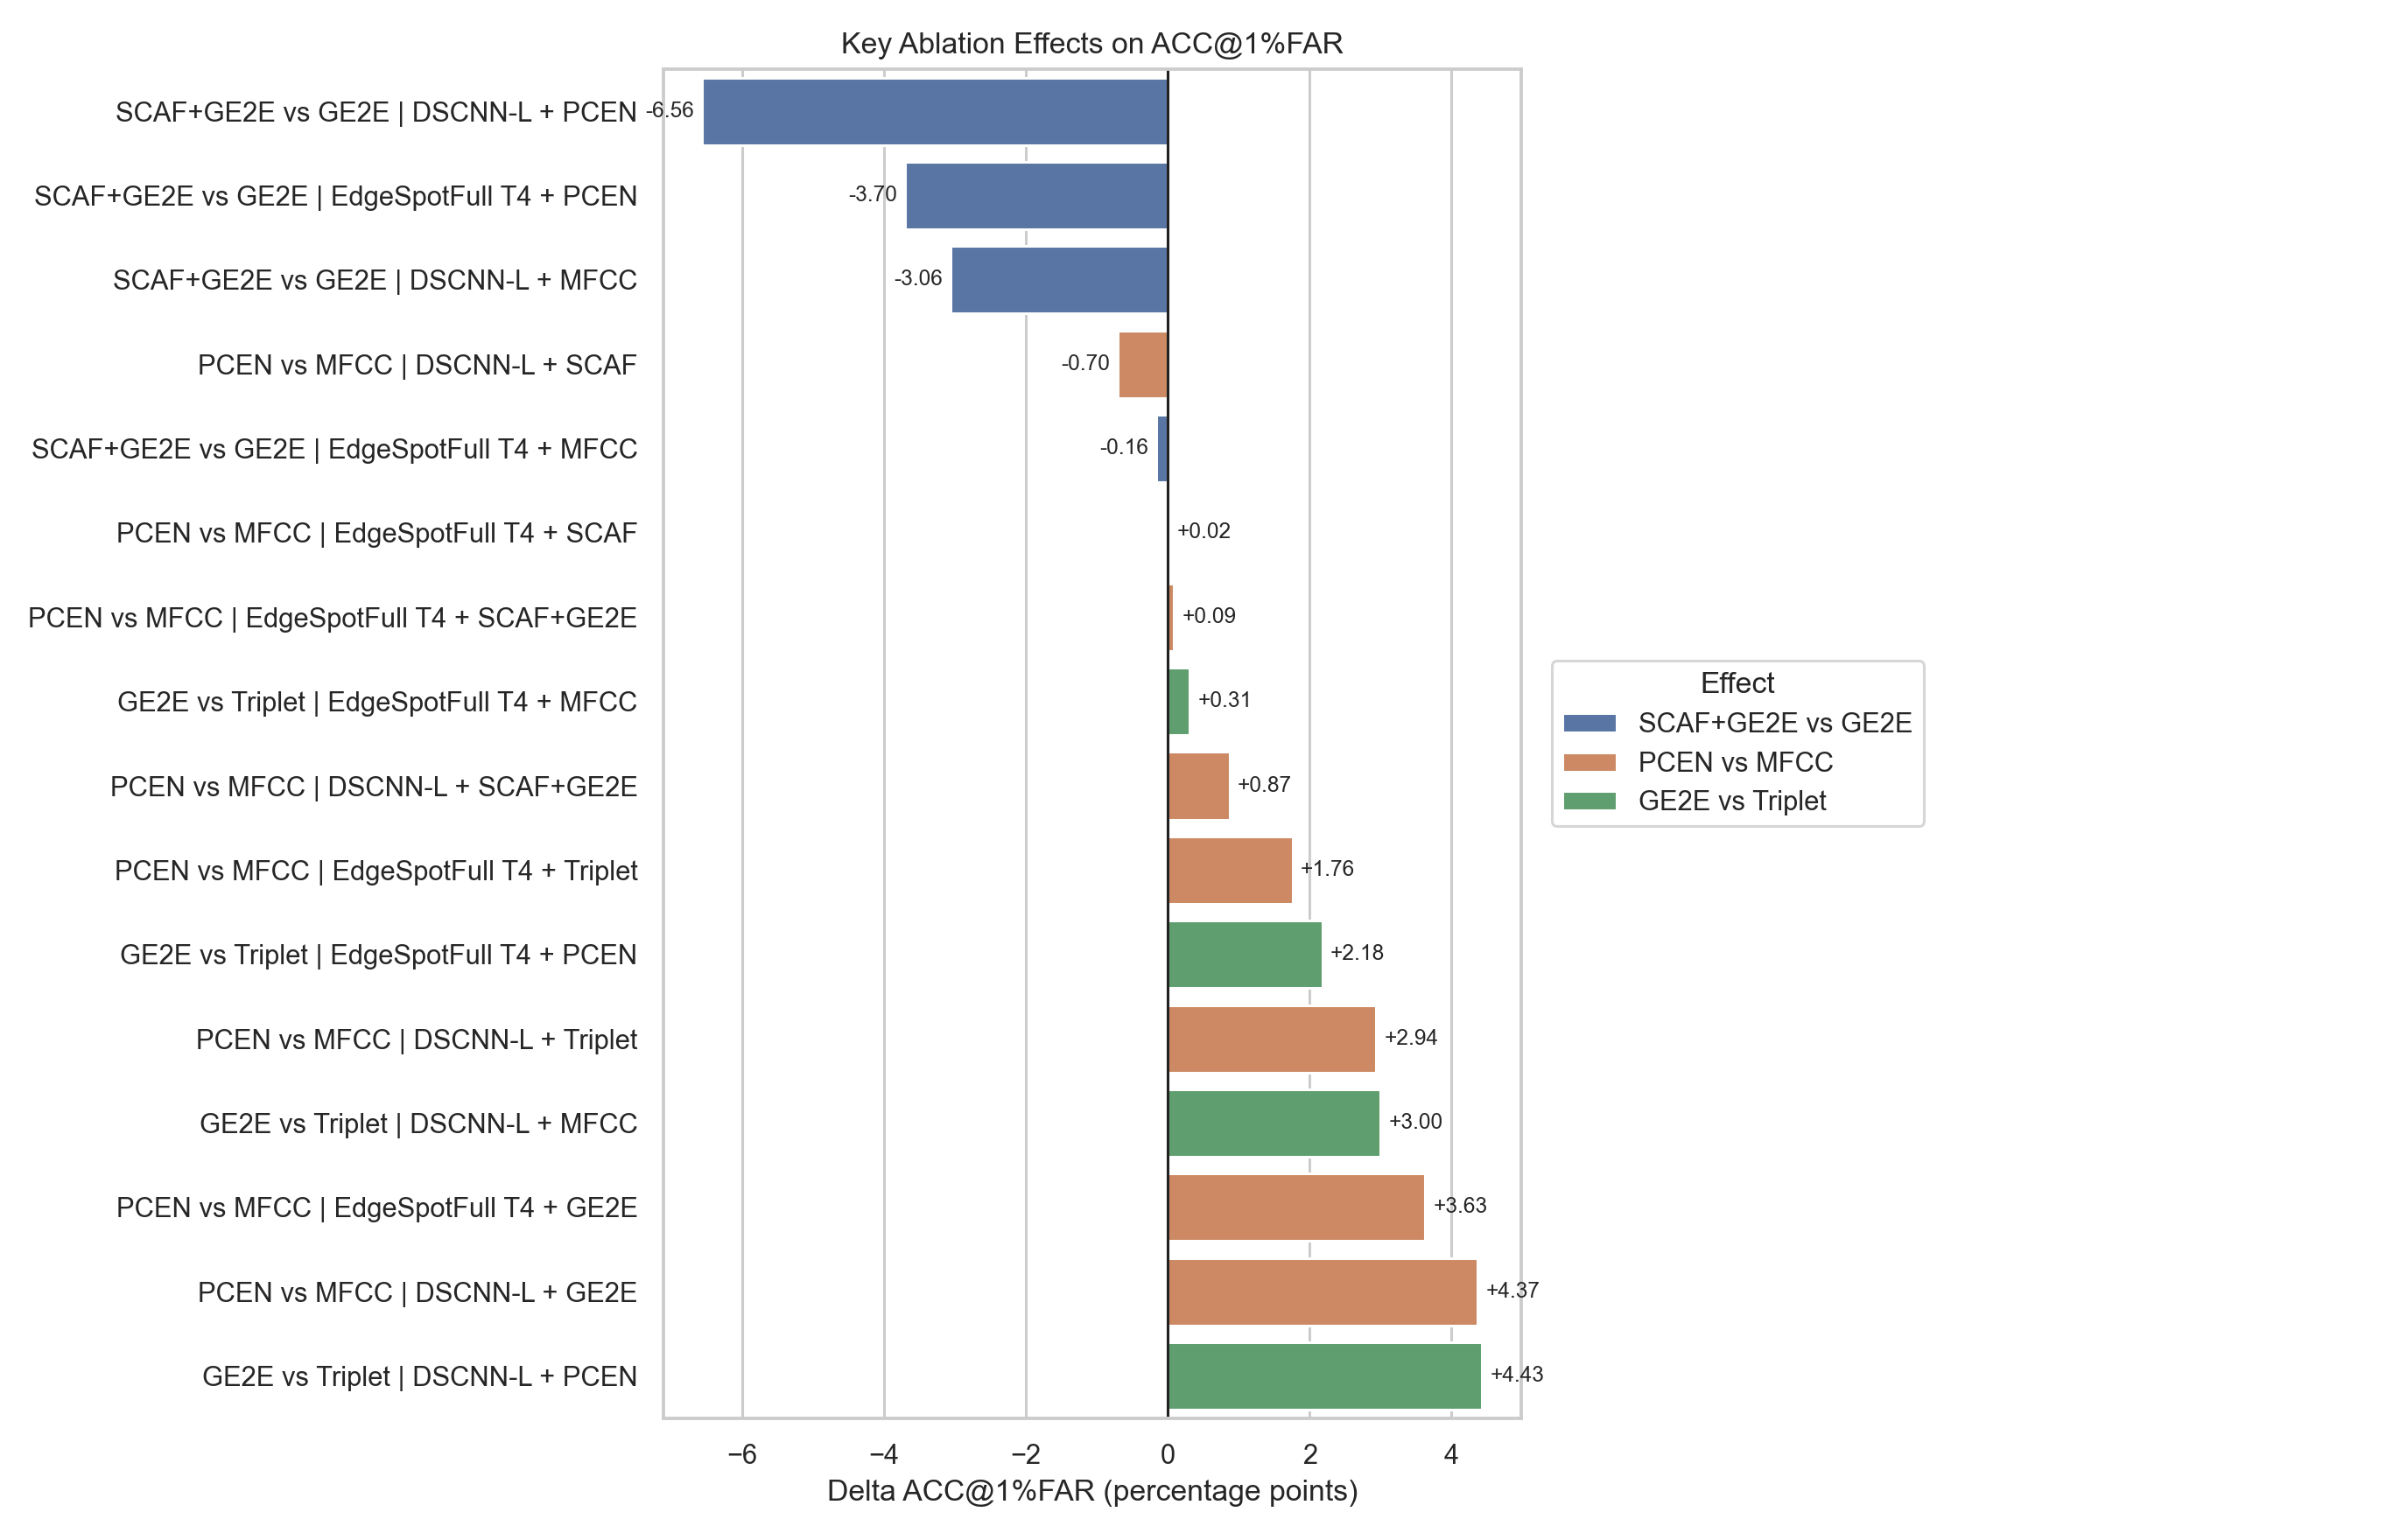
\includegraphics[width=0.92\linewidth]{res_effect_deltas.png}
\caption{Key paired effect deltas. PCEN and GE2E are the two consistent
improvements across backbones.}
\label{fig:deltas}
\end{figure}

\subsection{Q2: Scale --- saturation and the SCAF collapse}\label{sec:res-q2}

\paragraph{Accuracy saturates near 2\,M clips.}
Figure~\ref{fig:saturation} and Table~\ref{tab:scale} sweep the per-word cap for
the best front-end/loss (PCEN$+$GE2E). There is a large jump between cap-50 and
cap-220 ($+3.55$ ACC for DSCNN, $+3.79$ for EdgeSpot at 5\% FAR) and a flat region
from cap-220 to cap-620. Accuracy is effectively data-saturated at $\sim$2\,M
training clips: beyond this point, more clips of the same words yield negligible
cross-corpus gains.

\begin{figure}[t]
\centering
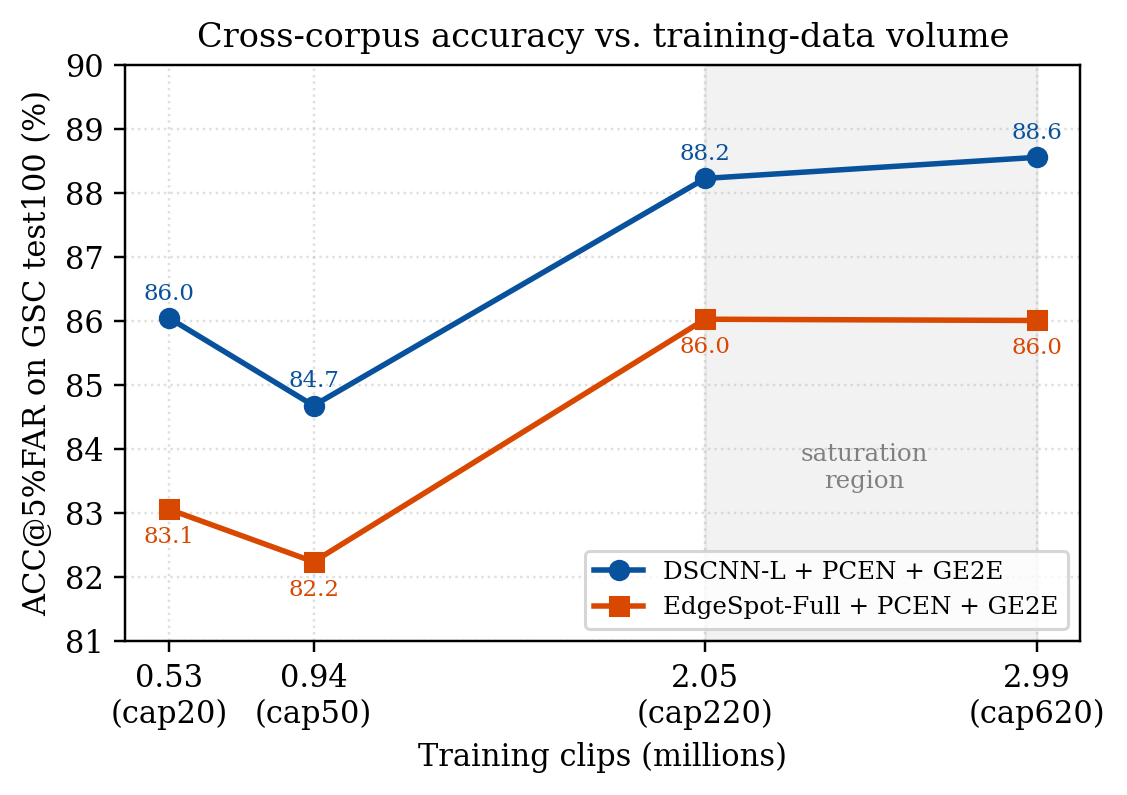
\includegraphics[width=0.80\linewidth]{fig_data_saturation.png}
\caption{Cross-corpus accuracy vs.\ training-data volume (per-word caps).
Performance saturates near $\sim$2\,M clips (shaded).}
\label{fig:saturation}
\end{figure}

\begin{table}[t]
\centering
\caption{Data-scale sweep (PCEN$+$GE2E), GSC test100. ACC at 5\% FAR.}
\label{tab:scale}
\small
\begin{tabular}{l c r r r r}
\toprule
\textbf{Encoder} & \textbf{Cap} & ACC$_{5\%}$ & AUC & EER & F1\\
\midrule
\multirow{4}{*}{DSCNN-L}
 & 20  & 86.05 & 91.57 & 16.25 & 75.90 \\
 & 50  & 84.68 & 90.45 & 17.42 & 74.34 \\
 & 220 & 88.23 & 93.87 & 12.78 & 80.67 \\
 & 620 & \textbf{88.56} & \textbf{94.04} & \textbf{12.53} & \textbf{81.02} \\
\midrule
\multirow{4}{*}{EdgeSpot}
 & 20  & 83.06 & 87.22 & 20.40 & 70.46 \\
 & 50  & 82.24 & 87.74 & 20.19 & 70.73 \\
 & 220 & \textbf{86.03} & 91.31 & 16.47 & 75.61 \\
 & 620 & 86.01 & \textbf{91.34} & 16.64 & 75.38 \\
\bottomrule
\end{tabular}
\end{table}

\paragraph{The SCAF collapse at 37k classes.}
The most striking result of the scale study is a qualitative failure. On the
31-class micro-set and the $\sim$500-class Top-500 split, SCAF and SCAF$+$GE2E are
excellent (AUC $\approx 95$). However, on the full $37{,}387$-class vocabulary
with the default SCAF weight of 1.0, training collapses from epoch~2: validation
AUC pins at 0.5000, the in-episode GE2E accuracy falls to $\approx 0.033$
($\approx 1/30$, chance), and the GSC metrics become degenerate (AUC 50, F1 0,
FRR$=$100\%, keyword ACC 9.09\%). The mechanism is a gradient-magnitude
imbalance: the sub-center ArcFace logit scale ($s{=}30$) multiplied across
$\sim$$3.7\times10^4$ classes produces a classification gradient that dwarfs the
centroid/cosine terms, driving all embeddings to a trivial solution. The same
hybrid does \emph{not} collapse under KD, where the SCAF weight is
$5\times10^{-5}$. Practical remedies we verify are: (i) reduce the SCAF weight to
$\sim$$5\times10^{-5}$, (ii) warm up the margin/scale, or (iii) drop the
classification term and use GE2E or KD. This is a cautionary result:
angular-margin classification losses that are state-of-the-art at $10^2$--$10^3$
classes do not transfer naively to $10^4$-class word embedding.

\TODOfig{Collapse curve for the full-vocabulary SCAF$+$GE2E run (validation AUC
pinned at 0.50 from epoch~2; in-episode accuracy $\sim$0.033). This run's logs are
not in the local repo, so it must be re-run on Colab (see the figures runbook).
Plot it with \code{make\_training\_curves.py} and save as
\code{assets/scaf\_collapse.png}.}

\subsection{Q3: Knowledge distillation trades teacher knowledge for data}\label{sec:res-q3}

Table~\ref{tab:kd} distils a frozen Wav2Vec\,2.0 teacher into the compact EdgeSpot
student. At cap-50, KD improves every metric over GE2E ($+3.60$ ACC@1\%FAR,
$-4.78$ EER, $+6.31$ F1) and, strikingly, KD at cap-50 matches GE2E at cap-220 ---
the same accuracy with roughly half the training clips. KD also saturates early,
indicating that the teacher injects most of its useful inductive bias from limited
data.

\begin{table}[t]
\centering
\caption{Knowledge distillation vs.\ GE2E (EdgeSpot student), GSC test100.}
\label{tab:kd}
\small
\begin{tabular}{l l r r r r}
\toprule
\textbf{Cap} & \textbf{Loss} & ACC$_{1\%}$ & ACC$_{5\%}$ & EER & F1\\
\midrule
50  & GE2E & 77.14 & 82.24 & 20.19 & 70.73 \\
\rowcolor{blue!7}
50  & KD   & \textbf{80.74} & \textbf{85.82} & \textbf{15.41} & \textbf{77.04} \\
220 & GE2E & --    & 86.03 & 16.47 & 75.61 \\
220 & KD   & 80.82 & 85.90 & 15.36 & 77.10 \\
\bottomrule
\end{tabular}
\end{table}

\subsection{Q4: Best deployable systems}\label{sec:res-q4}

Table~\ref{tab:final} consolidates the strongest configurations per data regime,
and Figures~\ref{fig:detcurve}--\ref{fig:heatmap} visualise the headline operating
point. Three points stand out:
\begin{itemize}[leftmargin=1.3em,itemsep=2pt]
\item \textbf{Best overall:} DSCNN-L$+$PCEN$+$GE2E (cap-620) reaches
$\mathbf{86.36\pm1.29}$ ACC@1\%FAR and $89.93\pm0.65$ at 5\% FAR, with AUC 95.21,
EER 11.32, F1 82.73, keyword ACC 92.92\%.
\item \textbf{Best compact:} EdgeSpot-Full$+$PCEN$+$GE2E (cap-620, ep300
composite) reaches $\mathbf{82.87\pm1.22}$ ACC@1\%FAR at 0.131\,M parameters ---
within $\sim$3.5 points of the best system at one third the size, and competitive
with (slightly above the mean of) the EdgeSpot-4 literature reference
($\sim$82\% ACC@1\%FAR, $\sim$128k params).
\item \textbf{Best small-vocabulary:} on the reduced Top-500 split, the
EdgeSpot$+$PCEN$+$SCAF$+$GE2E hybrid is the strongest compact model
($85.62\pm1.04$ ACC@1\%FAR, AUC 95.34), confirming the hybrid is excellent
\emph{when the class count is small enough not to trigger the collapse}.
\end{itemize}

\begin{table}[t]
\centering
\caption{Consolidated best systems across data regimes (GSC test100, 10-shot, 100
runs). ``coll.''$=$ degenerate collapse.}
\label{tab:final}
\small
\setlength{\tabcolsep}{4pt}
\begin{tabular}{l l l c r r r r r r}
\toprule
\textbf{Regime} & \textbf{Encoder} & \textbf{Loss} & \textbf{Params} &
ACC$_{1\%}$ & ACC$_{5\%}$ & AUC & EER & F1 & KW\\
\midrule
Micro (31)    & EdgeSpot & SCAF+GE2E      & 0.131M & 84.61 & 86.12 & 95.61 & 11.54 & 82.41 & 77.66 \\
Top-500       & EdgeSpot & SCAF+GE2E\,ep13& 0.131M & 85.62 & 88.79 & 95.34 & 11.51 & 82.45 & 90.44 \\
Top-500       & DSCNN-L  & GE2E           & 0.413M & 81.55 & 86.56 & 93.17 & 14.00 & 78.97 & 88.62 \\
Full cap20    & DSCNN-L  & GE2E           & 0.413M & 82.10 & 86.05 & 91.57 & 16.25 & 75.90 & 88.90 \\
Full cap220   & DSCNN-L  & GE2E           & 0.413M & --    & 88.23 & 93.87 & 12.78 & 80.67 & 89.82 \\
\rowcolor{blue!7}
Full cap620   & DSCNN-L  & GE2E\,ep300    & 0.413M & \textbf{86.36} & \textbf{89.93} & \textbf{95.21} & \textbf{11.32} & \textbf{82.73} & \textbf{92.92} \\
Full cap620   & EdgeSpot & GE2E\,ep300    & 0.131M & 82.87 & 86.76 & 92.41 & 14.82 & 77.85 & 87.29 \\
Full cap50    & EdgeSpot & KD             & 0.131M & 80.74 & 85.82 & 91.19 & 15.41 & 77.04 & 87.95 \\
Full cap220   & EdgeSpot & SCAF+GE2E      & 0.131M & coll. & coll. & 50.00 & 50.00 & coll. & 9.09 \\
\bottomrule
\end{tabular}
\end{table}

\begin{figure}[t]
\centering
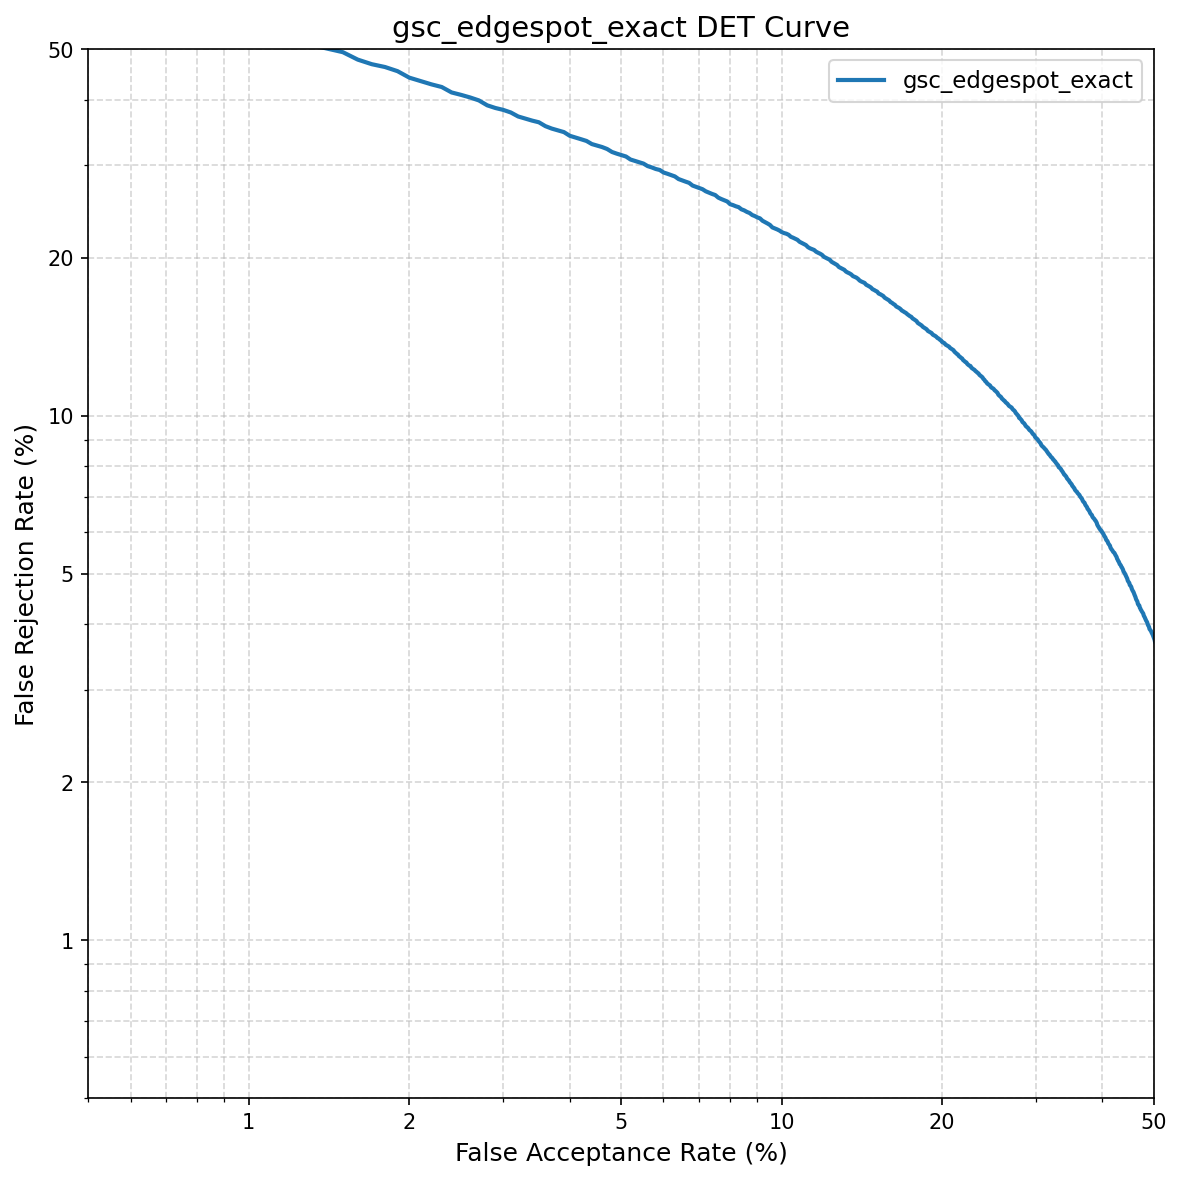
\includegraphics[width=0.62\linewidth]{res_det_dscnn.png}
\caption{Detection-error-tradeoff (DET) curve of the best overall system
(DSCNN-L$+$PCEN$+$GE2E).}
\label{fig:detcurve}
\end{figure}

\begin{figure}[t]
\centering
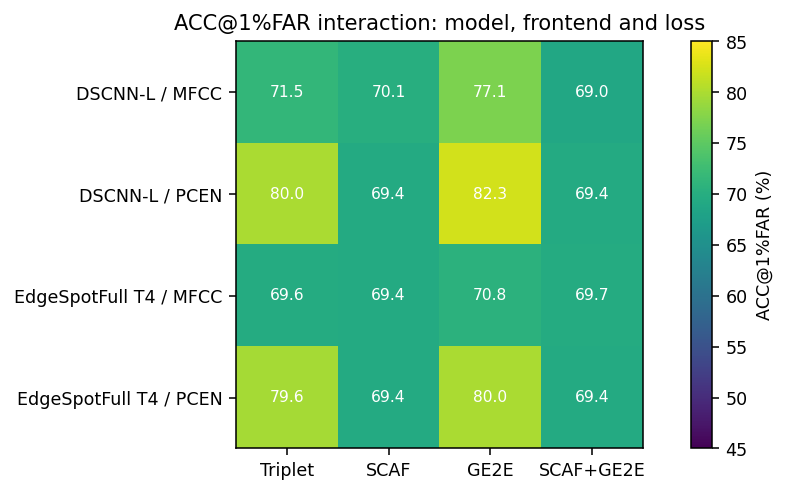
\includegraphics[width=0.7\linewidth]{res_cap620_heatmap.png}
\caption{ACC@1\%FAR heat map over the cap-620 configurations.}
\label{fig:heatmap}
\end{figure}

\paragraph{Accuracy vs.\ model size.}
Figure~\ref{fig:tradeoff} places the systems on the accuracy--size plane. DSCNN-L
leads on accuracy; EdgeSpot-Full reaches a competitive point at one third the
parameters; KD lifts the compact model further at low data.

\begin{figure}[t]
\centering
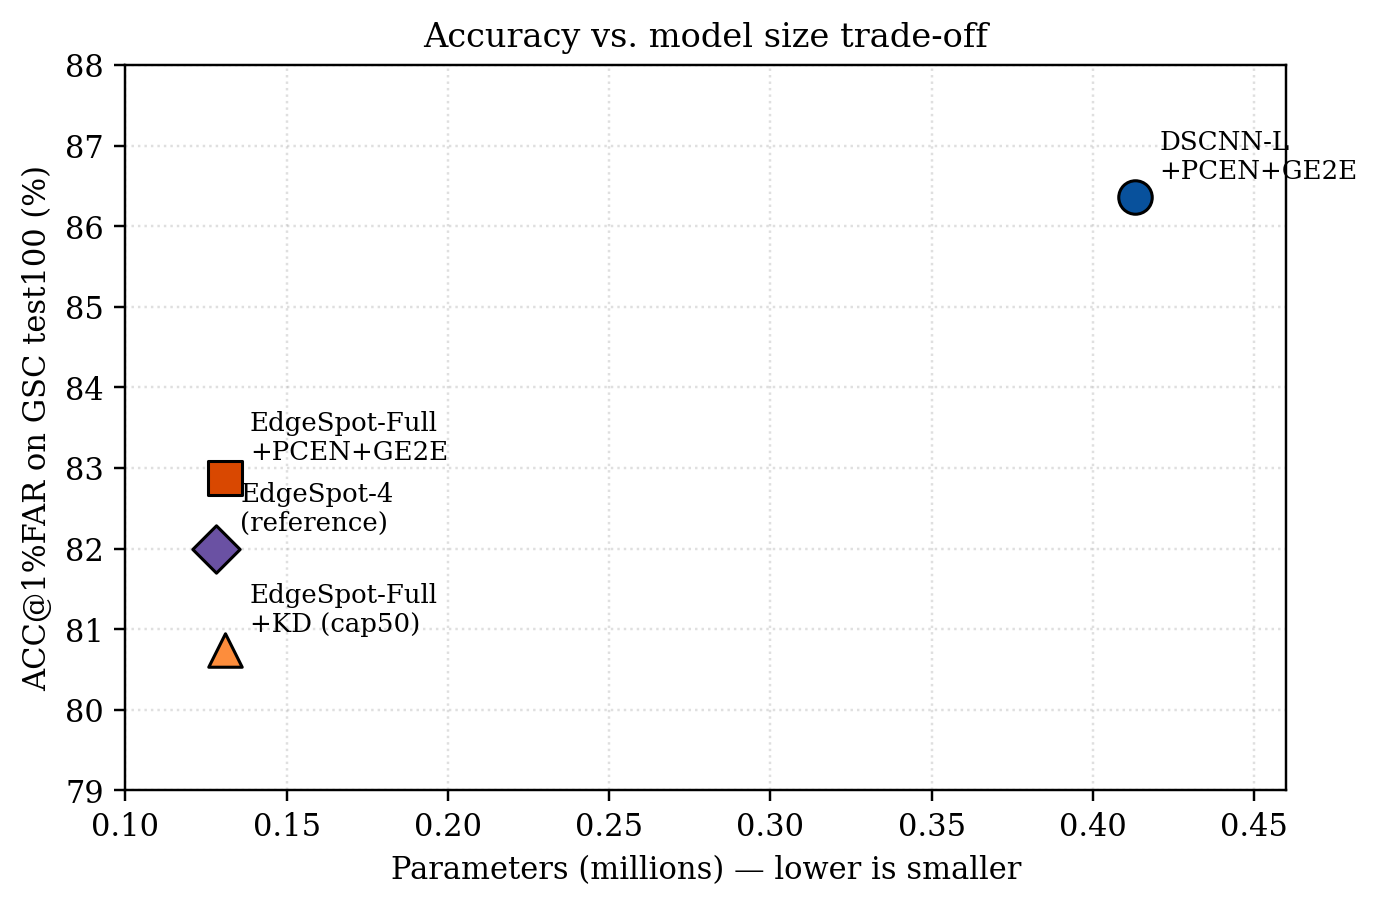
\includegraphics[width=0.78\linewidth]{fig_model_tradeoff.png}
\caption{Accuracy vs.\ model size. The compact EdgeSpot-Full sits within a few
points of the larger DSCNN-L at one third the parameters.}
\label{fig:tradeoff}
\end{figure}

\subsection{Inference on long audio}\label{sec:res-inference}

To verify the system end-to-end --- not only on isolated test clips --- we enrol
prototypes for 17 keywords (10 shots each from GSC) and run nearest-prototype
inference over a real, continuously spoken multi-word recording.
Figure~\ref{fig:longinfer} overlays the predicted keyword and its prototype
distance on the waveform for the first 16 spoken segments. The model correctly
identifies $15/16$ segments ($\approx$94\%); the single error (``sheila'', a long,
rare name) also has the largest prototype distance --- exactly the signal the
open-set threshold uses to flag low-confidence detections.
Figure~\ref{fig:interaction} shows the front-end$\times$loss interaction: the
PCEN$+$GE2E cell dominates, while classification-only cells degrade at full
vocabulary scale.

\begin{figure}[t]
\centering
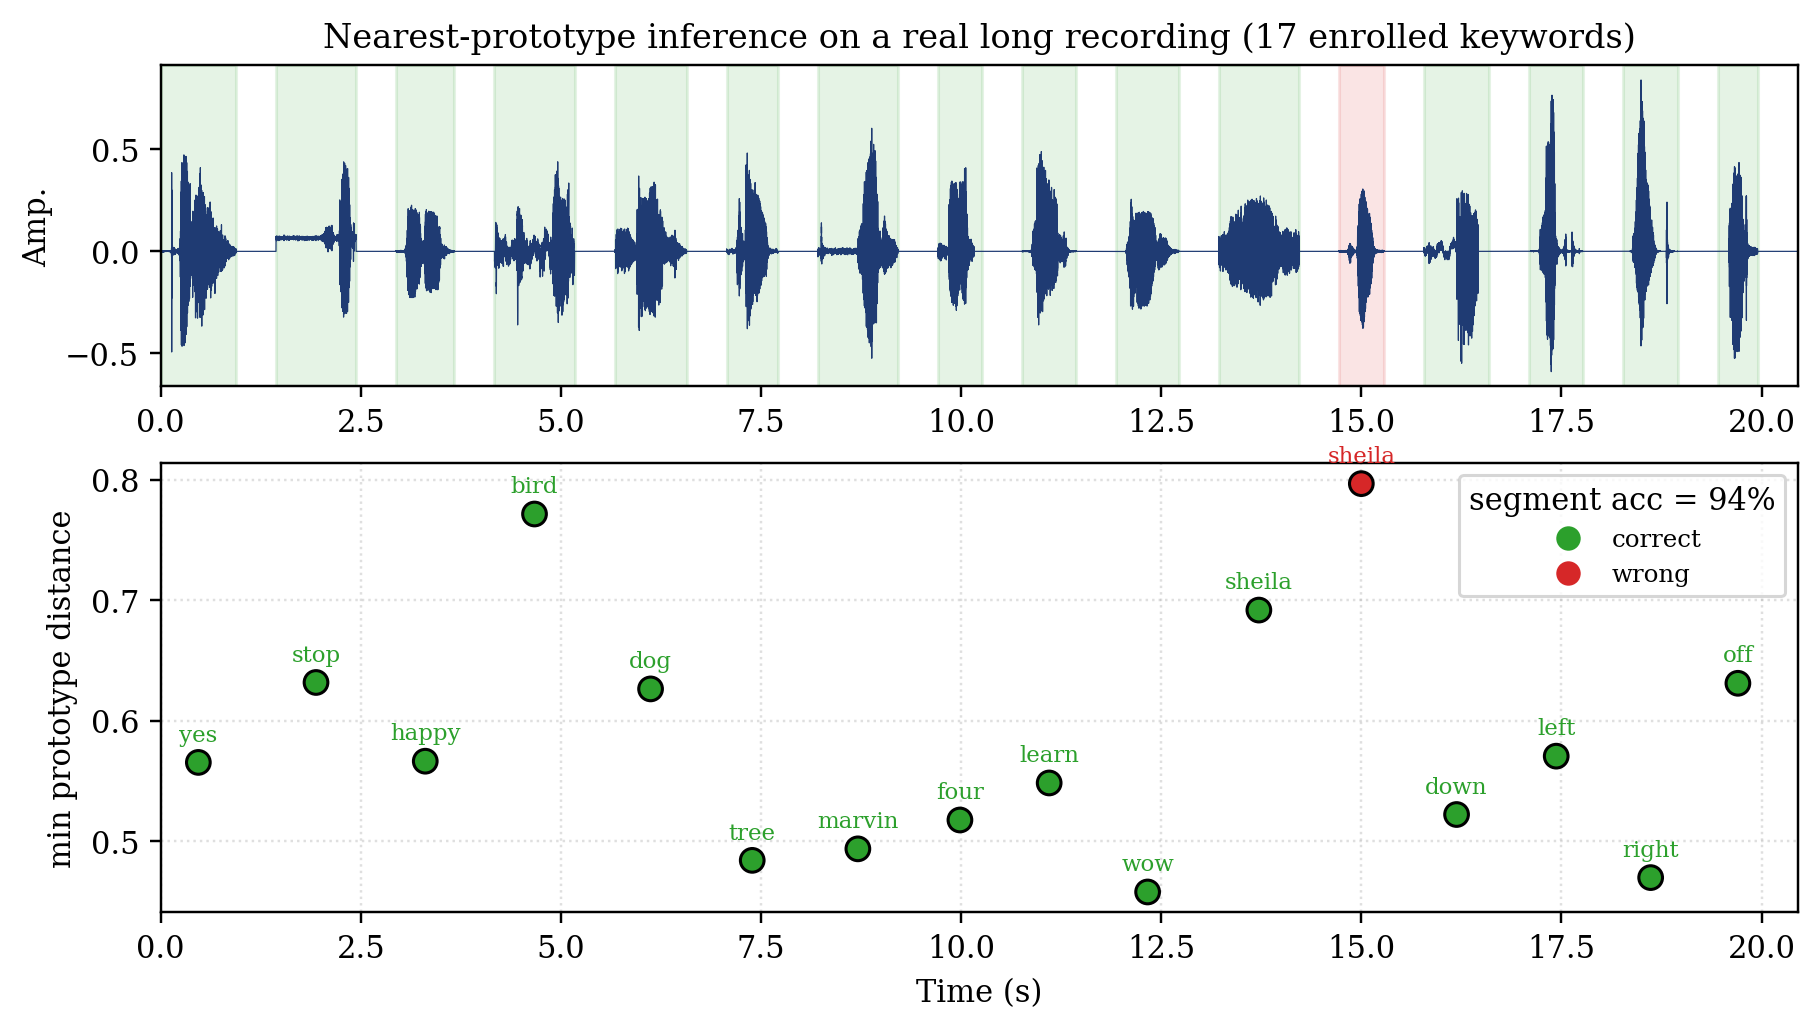
\includegraphics[width=0.98\linewidth]{fig_long_inference.png}
\caption{Nearest-prototype inference on a real long recording. Top: waveform with
per-segment correct (green) / wrong (red) shading. Bottom: minimum prototype
distance and predicted keyword per segment.}
\label{fig:longinfer}
\end{figure}

\begin{figure}[t]
\centering
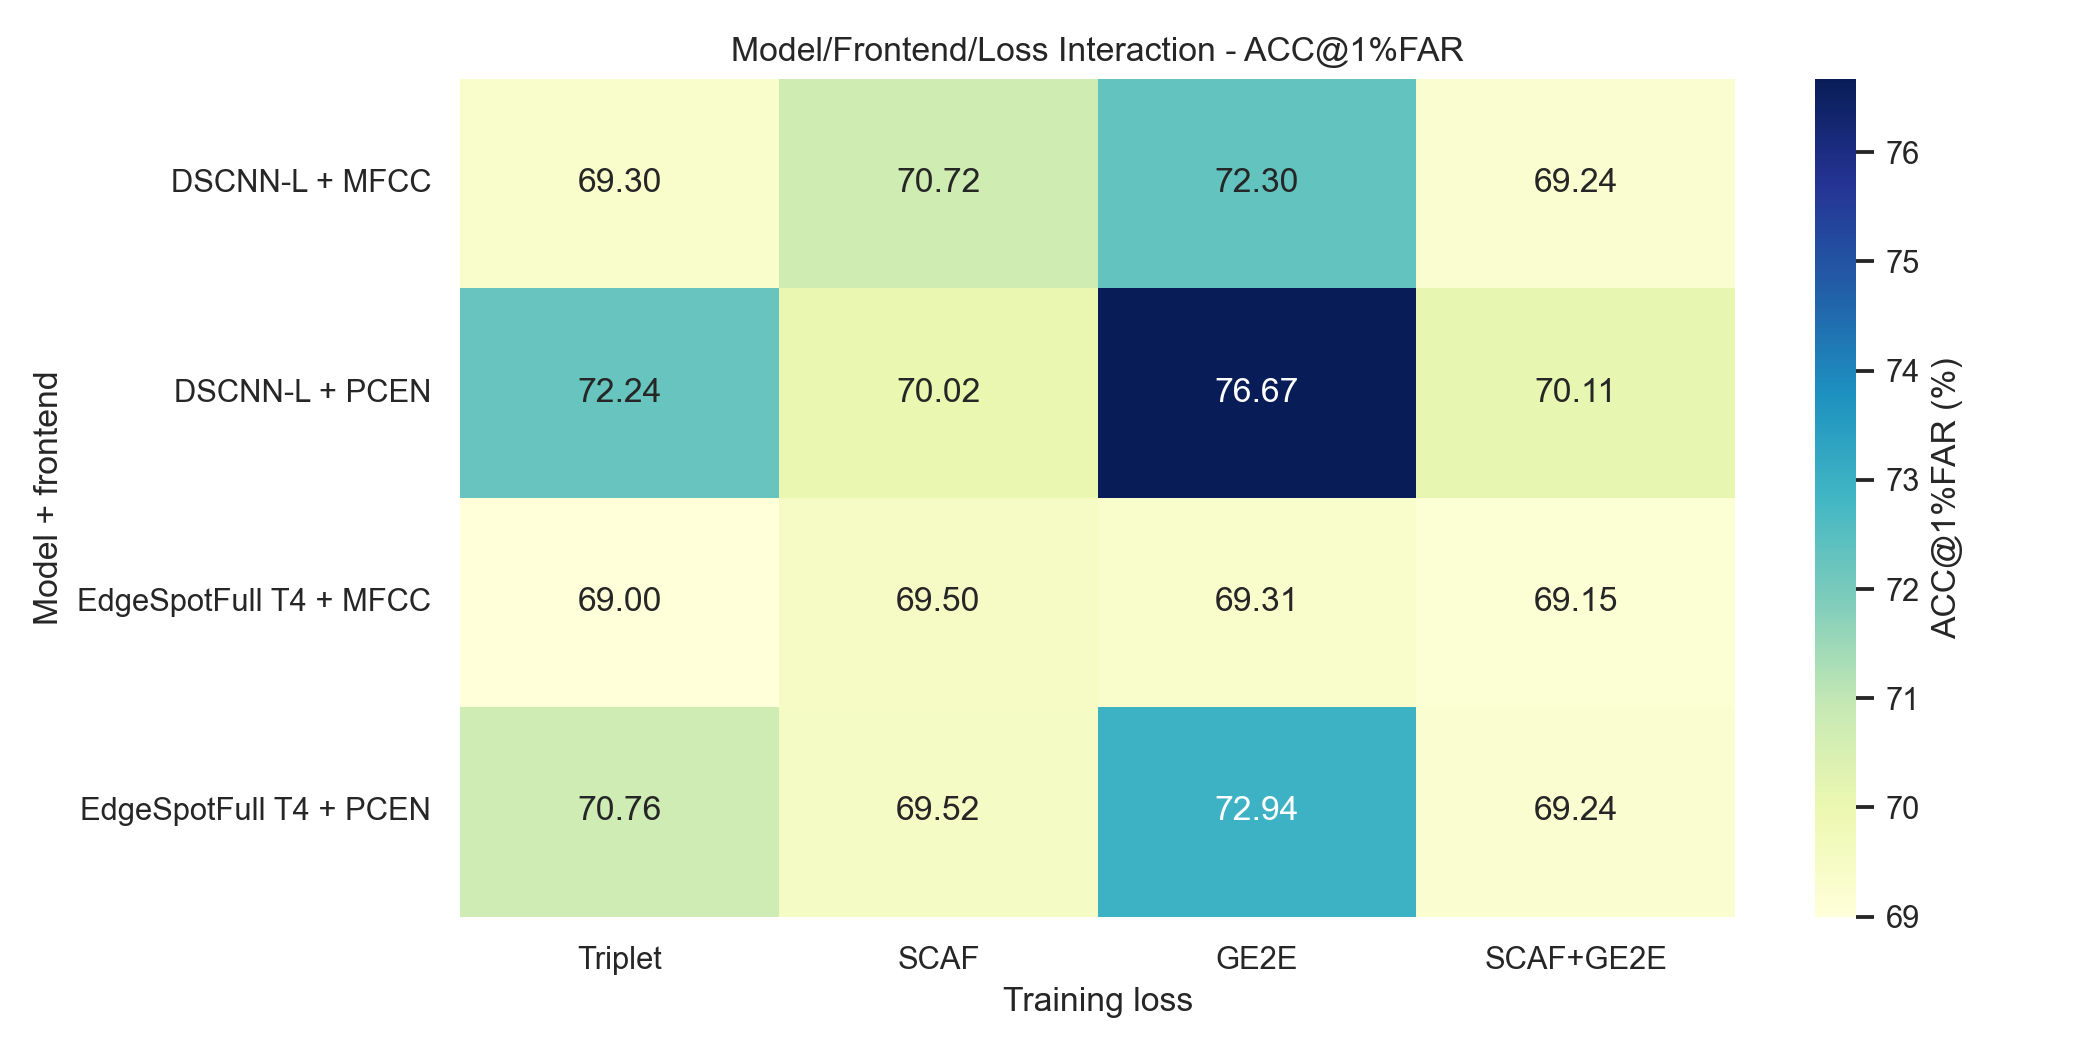
\includegraphics[width=0.82\linewidth]{res_interaction_heatmap.png}
\caption{Front-end $\times$ loss interaction (ACC@1\%FAR). The PCEN$+$GE2E cell
dominates; classification-only cells degrade at full vocabulary scale.}
\label{fig:interaction}
\end{figure}

\paragraph{Reproducibility note on data regimes.}
Within full-vocabulary results, three cap-620 runs use different episode budgets
(a 40-epoch fixed screen, a 1000-episode saturation run, and a 300-episode
composite-selection development run). They must not be conflated; each table row
is drawn from a single consistent run, with the budget stated where it matters.

%==============================================================================
\section{Conclusion and Perspective}\label{sec:conclusion}

\subsection{Current status}\label{sec:status}

This thesis set out to build a keyword-spotting system that escapes the two
structural limits of classical wake-word engines --- a frozen vocabulary and the
inability to abstain --- and to understand, rather than merely report, what makes
such a system work as the training vocabulary grows. We delivered a complete,
reproducible, dependency-light pipeline: two compact encoders (DSCNN-L at
$\approx$0.41\,M and EdgeSpot-Full at $\approx$0.13\,M parameters), three feature
front-ends, four metric-learning objectives, four open-set rejection heads, a CPU
streaming engine, and an offline web demonstrator. Every system is trained on
MSWC English and evaluated cross-corpus on GSC v2 under a single strict 10-shot
protocol with 100 randomised runs, so the numbers compare fairly.

The headline outcome is that few-shot open-set KWS is viable and even strong at
true vocabulary scale: training once on $37{,}387$ words, the best configuration
(DSCNN-L $+$ PCEN $+$ GE2E) reaches $86.36\%$ open-set accuracy at a strict $1\%$
false-accept rate and $95.21$ AUC on a corpus it was never trained on, while a
three-times-smaller edge model (EdgeSpot-Full $+$ PCEN $+$ GE2E) stays within a
few points at $82.87\%$. A user can define an arbitrary keyword set from ten
examples per word, with no retraining, and the system can decline to answer on
unknown speech and silence.

\subsection{What is good, what is weak}\label{sec:goodbad}

\paragraph{What works.} Three findings are robust and transferable. (1) The
trainable PCEN front-end is the most reliable single improvement, and it helps the
smaller encoder most --- a useful lever precisely where the parameter budget is
tightest. (2) The centroid GE2E objective, which optimises the same
enrol-then-match computation used at deployment, consistently beats both triplet
and classification objectives for open-set generalisation. (3) A frozen
Wav2Vec\,2.0 teacher distilled with a simple cosine loss lets the compact model
reach GE2E-level accuracy with roughly half the data.

\paragraph{What is weak.} The clearest negative result is the collapse of the
sub-center ArcFace (SCAF) classification objective at $10^4$-class scale: a loss
that is excellent on tens to hundreds of classes drives the embedding to a trivial
solution on tens of thousands of classes unless its weight is cut by four orders
of magnitude. Two further limitations bound the present claims. First, the
ACC@FAR/FRR@FAR operating points are read from the evaluation ROC (an oracle
threshold) rather than transferred from an independent calibration split; we
mitigate this by always co-reporting threshold-free AUC/EER/F1, but a calibrated,
deployment-time threshold study is still owed. Second, enrolment is fixed at
$k{=}10$ shots and the streaming latency figures are design budgets, not measured
field benchmarks, and there is no quantitative denoising ablation.

\subsection{Future work}\label{sec:future}

Four directions follow directly from the limitations above.
(1) \emph{$k$-shot sensitivity:} sweep $k\in\{1,3,5,10\}$ to chart the
accuracy-vs-enrolment-effort curve, which is the metric end users actually feel.
(2) \emph{Calibrated thresholds:} learn or transfer the open-set threshold from a
held-out split and report deployment-realistic ACC@FAR, closing the oracle gap.
(3) \emph{On-device benchmark:} measure end-to-end latency, false-alarms-per-hour,
and miss-rate on target hardware, plus an SNR-sweep denoising ablation.
(4) \emph{Stabilising classification at scale:} margin/scale warm-up, curriculum,
or sub-center pruning to recover the discriminative power of angular-margin losses
without the collapse.

In summary, the thesis demonstrates a deployable, retraining-free, open-set
keyword spotter and, just as importantly, a clear empirical map of which design
choices help, where they saturate, and where they fail as the problem scales.

%==============================================================================
\begin{thebibliography}{99}
\footnotesize

\bibitem{zhang2017hello} Y.~Zhang, N.~Suda, L.~Lai, and V.~Chandra,
``Hello edge: Keyword spotting on microcontrollers,'' \emph{arXiv:1711.07128}, 2017.
\bibitem{kim2021bcresnet} B.~Kim, S.~Chang, J.~Lee, and D.~Sung,
``Broadcasted residual learning for efficient keyword spotting,'' \emph{Interspeech}, 2021.
\bibitem{snell2017prototypical} J.~Snell, K.~Swersky, and R.~Zemel,
``Prototypical networks for few-shot learning,'' \emph{NeurIPS}, 2017.
\bibitem{schroff2015facenet} F.~Schroff, D.~Kalenichenko, and J.~Philbin,
``FaceNet: A unified embedding for face recognition and clustering,'' \emph{CVPR}, 2015.
\bibitem{wan2018ge2e} L.~Wan, Q.~Wang, A.~Papir, and I.~L.~Moreno,
``Generalized end-to-end loss for speaker verification,'' \emph{ICASSP}, 2018.
\bibitem{deng2019arcface} J.~Deng, J.~Guo, N.~Xue, and S.~Zafeiriou,
``ArcFace: Additive angular margin loss for deep face recognition,'' \emph{CVPR}, 2019.
\bibitem{deng2020subcenter} J.~Deng, J.~Guo, T.~Liu, M.~Gong, and S.~Zafeiriou,
``Sub-center ArcFace: Boosting face recognition by large-scale noisy web faces,'' \emph{ECCV}, 2020.
\bibitem{bendale2016openmax} A.~Bendale and T.~E.~Boult,
``Towards open set deep networks,'' \emph{CVPR}, 2016.
\bibitem{liu2020energy} W.~Liu, X.~Wang, J.~Owens, and Y.~Li,
``Energy-based out-of-distribution detection,'' \emph{NeurIPS}, 2020.
\bibitem{wang2017trainable} Y.~Wang, P.~Getreuer, T.~Hughes, R.~F.~Lyon, and R.~A.~Saurous,
``Trainable frontend for robust and far-field keyword spotting,'' \emph{ICASSP}, 2017.
\bibitem{baevski2020wav2vec} A.~Baevski, H.~Zhou, A.~Mohamed, and M.~Auli,
``wav2vec 2.0: A framework for self-supervised learning of speech representations,'' \emph{NeurIPS}, 2020.
\bibitem{mazumder2021mswc} M.~Mazumder \emph{et al.},
``Multilingual Spoken Words Corpus,'' \emph{NeurIPS Datasets and Benchmarks}, 2021.
\bibitem{warden2018speech} P.~Warden,
``Speech Commands: A dataset for limited-vocabulary speech recognition,'' \emph{arXiv:1804.03209}, 2018.

\end{thebibliography}

%==============================================================================
\newpage
\appendix
\renewcommand{\thesection}{Appendix \Alph{section}:}
\setcounter{section}{0}

\section{Streaming decision state machine}\label{app:sm}

The streaming detector stabilises raw per-window candidates into clean events
with majority-vote smoothing, a top-2 margin check, and a cooldown:

\begin{enumerate}[leftmargin=1.8em,itemsep=1pt]
\item Maintain a short ring buffer of recent candidates and the timestamp
$t_{\text{last}}$ of the last emitted event.
\item For each candidate $c$ with span $[t_s,t_e]$: if $t_s - t_{\text{last}} <
C$ (cooldown), emit \textsc{cooldown} and continue.
\item If $c$ is not detected, or its keyword is \code{unknown}, or its top-2
margin $<m_{\min}$: clear the buffer, emit \textsc{rejected}, and continue.
\item Otherwise push $c$ and let $k^\star$ be the majority keyword in the buffer.
\item If $\text{votes}(k^\star)\ge V$: pick the highest-confidence candidate of
$k^\star$, set $t_{\text{last}}$ to its end, clear the buffer, and emit
\textsc{detected}$(k^\star)$; else emit \textsc{scoring}.
\end{enumerate}

The server runs ingestion and inference as a non-blocking producer/consumer pair
with at most one inference in flight, so detection latency stays bounded to about
one process cycle even when the model cannot keep up with the realtime chunk rate.

\section{Reproducibility summary}\label{app:repro}

\begin{itemize}[leftmargin=1.4em,itemsep=1pt]
\item \textbf{Audio:} 16\,kHz mono, 1\,s windows; MFCC $(1,47,10)$ or log-mel
$(1,40,101)$; optional trainable PCEN.
\item \textbf{Episodes:} 30 classes $\times$ 20 utterances; DEMAND noise
($p{=}0.5$, SNR $[0,10]$\,dB) $+$ SpecAugment $+$ gain/time-shift.
\item \textbf{Optimisation:} Adam ($10^{-3}$, weight decay $10^{-4}$), grad-clip
$5.0$, cosine-annealing warm restarts, seed 42, cuDNN deterministic.
\item \textbf{Evaluation:} GSC v2, 10-shot, 11 positive / 25 unknown classes,
100 runs (test100); metrics ACC@\{1,5\}\%FAR, AUC, EER, FRR@FAR, keyword ACC, F1.
\item \textbf{Best checkpoints:} DSCNN-L$+$PCEN$+$GE2E (best overall) and
EdgeSpot-Full\,$\tau{=}4$\,$+$PCEN$+$GE2E (best compact), cap-620, ep300 composite
selection by mean(ACC@1\%FAR, AUC, F1) on GSC-dev.
\end{itemize}

\end{document}
